% !TeX document-id = {bd69b656-54da-46f4-a905-dc662e17f4b3}
% !TeX TXS-program:compile = txs:///pdflatex/[-shell-escape -halt-on-error]

\documentclass[fontsize=10pt,openright,oneside,paper=a4,BCOR=1cm,numbers=noenddot,english]{scrbook}
% \documentclass[fontsize=10pt,openright,oneside,paper=a4,BCOR=1cm,numbers=noenddot,ngerman]{scrbook} % German

% Patch page headers to not be UPPER CASE
\makeatletter
\renewcommand\scr@chapter@after@hyperref@patch{}
\makeatother

\usepackage[top=3.5cm, bottom=3.5cm, left=3.0cm, right=4.0cm]{geometry}
\usepackage[T1]{fontenc}
\usepackage{lipsum}


%%%%%%%%%%%%%%%%%%%%%%%%%%%%%%%%%%%%%%%%%%%%%%%%%%%%%%%%%%%%
% Basic definitions, to be adjusted individually
\newcommand{\authornamefirst}{Ilnaz}
\newcommand{\authornamelast}{Tayebi}
\newcommand{\matrikelnummer}{107323}
\newcommand{\authorhomestreet}{Home number}
\newcommand{\authorpostalcodecity}{94032, Passau}

\newcommand{\worktitle}{Efficient Indexing of Raw Data Files}

\newcommand{\thesistype}{Master's Thesis}

\newcommand{\courseofstudies}{Computer Science}

\newcommand{\thesisdate}{\today}   %% in ISO 8601 format

\newcommand{\thesisprof}{Prof. Dr. Stefanie Scherzinger}
\newcommand{\thesisproftwo}{Prof. Dr. Harald Kosch}
\newcommand{\chair}{\mbox{Chair of Scalable Database Systems}}

\newcommand{\secondchair}{Chair of Distributed Information Systems}

% \newcommand{\advisor}{Your Advisor (usually not the professor)}


\newcommand{\contactprofone}{
\thesisprof \\
\chair \\
University of Passau \\
Email:~{\small \href{mailto:stefanie.scherzinger@uni-passau.de}{\texttt{stefanie.scherzinger@uni-passau.de}}}  \\
Web:~{\small
\url{https://www.fim.uni-passau.de/en/database-systems/}}\\}

% Only for master's thesis. Just comment these lines if you don't have or need a second supervisor.
\newcommand{\contactproftwo}{
\thesisproftwo \\
\secondchair \\
University of Passau \\ % German: Universität Passau \\
Email:~{\small \href{mailto:<second.prof>@uni-passau.de}{\texttt{Harald.Kosch@uni-passau.de}}}  \\
Web:~{\small
\url{https://www.fim.uni-passau.de/en/distributed-information-systems}}\\}


%\newcommand{\drosera}{\textit{Drosera}\xspace}
%%%%%%%%%%%%%%%%%%%%%%%%%%%%%%%%%%%%%%%%%%%%%%%%%%%%%%%%%%%%

% PACKAGES:

\usepackage{xcolor}
\usepackage{xargs}

%%%%%%%%%%%%%%%%%%%%%%%%%%%%%%%%%%%%%%%%%%%%%%%%%%%%%%%%%%%%%%%%%%%
%%%%%%%%%%%%%%%%%%%%%%%%% REMOVE ME LATER %%%%%%%%%%%%%%%%%%%%%%%%%
%%%%%%%%%%%%%%%%%%%%%%%%%%%%%%%%%%%%%%%%%%%%%%%%%%%%%%%%%%%%%%%%%%%
% Todo notes
\usepackage[colorinlistoftodos,prependcaption]{todonotes}
\makeatletter
\renewcommand{\todo}[2][]{\tikzexternaldisable\@todo[inline,#1]{#2}\tikzexternalenable}
\makeatother
%%%%%%%%%%%%%%%%%%%%%%%%%%%%%%%%%%%%%%%%%%%%%%%%%%%%%%%%%%%%%%%%%%%
%%%%%%%%%%%%%%%%%%%%%%%%% REMOVE ME LATER %%%%%%%%%%%%%%%%%%%%%%%%%
%%%%%%%%%%%%%%%%%%%%%%%%%%%%%%%%%%%%%%%%%%%%%%%%%%%%%%%%%%%%%%%%%%%

% Better unsrt style with support for DOIs and URLs
\usepackage[numbers]{natbib}
% Use better appendices
\usepackage{appendix}
% German paragraph skip
\usepackage{parskip}
% Encoding. Use utf8. We are now in the 21st century already :-)
\usepackage[utf8]{inputenc}
% Index-generation
\usepackage{makeidx}
% Einbinden von URLs:
\usepackage{url}
% Include Graphic-files:
\usepackage{graphicx}
% Include PDF links
\usepackage{listings}
\usepackage{float}
\usepackage{tikz}
\usepackage{pgfplots}
\usepackage{multirow}
%mathstuff
\usepackage[cmex10]{amsmath}
\usepackage{amsfonts}
\usepackage{amssymb}
\usepackage{amsthm}
\usepackage{longtable}
\usepackage{pifont}
\newcommand{\cmark}{\ding{51}}
\newcommand{\xmark}{\ding{55}}
\usepackage{pdfpages}
\usepackage{multicol}
\usepackage{xspace}
\usepackage{mathtools}
\usepackage{extarrows}
\usepackage{hhline}
\usepackage[shortlabels]{enumitem}
\usepackage{environ}
\usepackage{xifthen}
\usepackage{capt-of}
\usepackage{custom-style}
\usepackage{booktabs}
\usepackage{tabularx}
\usepackage{csquotes}

\newcounter{mtpage}
% Global footnote counter
\counterwithout{footnote}{chapter}

% hyperref for nice inner-PDF hyperlinks
\usepackage[pdftex,
bookmarks=true,
pdfauthor={{{\authornamefirst \authornamelast}}},
pdftitle={{{\worktitle}}},
hidelinks
]{hyperref}
% cleveref for even better own references
\usepackage[capitalise]{cleveref}

%%%%%%%%%%%%%%%%%%%%%%%%%%%%%%%%%%%%%%%%%%%%%%%%%%%%%%%%%%%%

% OTHER SETTINGS:
\pgfplotsset{
  compat=1.18,
  scaled y ticks=false,
}

% Pagestyle:
\pagestyle{headings}

% Avoid 'overhang':
\sloppy

% Choose language
\newcommand{\setlang}[1]{\selectlanguage{#1}\nonfrenchspacing}

% English...
\usepackage[english]{babel}
\setlang{english}
% ... or German?
%\usepackage[ngerman]{babel}
%\setlang{ngerman}

\usepackage[iso,english]{isodate} % Don't change the language here!

\usepackage[Bjornstrup]{fncychap}

\definecolor{bblue}{HTML}{00A2FF}
\definecolor{rred}{HTML}{FF2600}
\definecolor{ggreen}{HTML}{61D836}
\definecolor{ppurple}{HTML}{C24885}
\definecolor{oorange}{HTML}{F8BA00}
\definecolor{ggray}{HTML}{5F5F5F}
\definecolor{ppink}{HTML}{e81cbf}

% Tikz Externalize
\usetikzlibrary{external, backgrounds, shapes.geometric, arrows, positioning, fit, decorations.pathreplacing, shapes.multipart}

\tikzexternalize[prefix=cache/]

% Pretty listings
\usepackage[newfloat,cachedir=cache/]{minted}
\usepackage{xcolor} % to access the named colour LightGray
\definecolor{LightGray}{gray}{0.9}
\usepackage{caption}
\newenvironment{code}{\captionsetup{type=listing}}{}
\usepackage{subcaption}

% Automatic quotes
%\usepackage[autostyle]{csquotes}
%\MakeOuterQuote{"}

% Acronym

\usepackage{glossaries}
\makeglossaries

%%%%%%%%%%%%%%%%%%%%%%%%%Glossries%%%%%%%%%%%%%%%%%%%%%%%%%%%%%%%%%%% 


% ------------------------------------------------------------------------------------------
% Use this if-flag to show or hide the draft content
% ------------------------------------------------------------------------------------------
\newif\ifshow
\showtrue % \showtrue or \showfalse
% ------------------------------------------------------------------------------------------
\NewEnviron{revise}[1][red]{
  \ifshow
    \textcolor{#1}{\BODY}
  \fi
}
% ------------------------------------------------------------------------------------------


% Custom commands
\let\oldphi\phi
\let\phi\varphi
\let\oldepsilon\epsilon
\let\epsilon\varepsilon

% TITLE:

\begin{document}
\frontmatter
\thispagestyle{empty}
\newpage

\vspace{1cm}

\begin{center}
\begin{tabular}{lr}

\includegraphics[width=6.5cm]{img/logouni_en.png}
% 
\includegraphics[width=6.5cm]{img/logouni.png} % German
\end{tabular}

\vspace{3cm}
\Large University of Passau
% \Large Universität Passau % German
\\
\Large Faculty of Computer Science and Mathematics
% \Large Fakultät für Informatik und Mathematik % German
\\
\vspace{0.3cm}
\Large {\chair }
\\
\Large \thesisprof

\end{center}


\vspace{2.5cm}

\begin{center}
        % Master's thesis, Bachelor's thesis, Programming project
        {\Large \thesistype\\ in\\ \courseofstudies\\} 
\end{center}

\begin{center}
        \settowidth{\baselineskip}{0.4cm}
        {\LARGE \textbf{\worktitle}}
        \\
        {\Large
        \vspace{1cm}
        \authornamefirst~\authornamelast \\ \matrikelnummer \\
        }
\end{center}

\vfill {% \settowidth{\baselineskip}{0.2cm}

\vfill


{\large
\begin{tabular}[l]{llll}

Date:       & \thesisdate %%(\LaTeX{}$2_\epsilon$ run \today) % German: Datum:
\smallskip \\
Supervisors:   & \thesisprof \\ % German: Prüfer:
	& \thesisproftwo \\
% Advisor: & \advisor \\ % German: Betreuer:
\end{tabular}}
} \cleardoublepage
%%%%%%%%%%%%%%%%%%%%%%%%%%%%%%%%%%%%%%%%%%%%%%%%%%%%%%%%%%%%
~
\vfill

\textbf{Supervisor contacts:} \smallskip \\ % German: Kontaktdaten des Prüfers:
\contactprofone\\
\contactproftwo\\

\cleardoublepage
% MAIN PART:

% Acknowledgement. 
%!TEX root = ../thesis.tex

\thispagestyle{plain}

\section*{Acknowlegment}
First of all, I would like to thank my supervisor, Prof. Dr. Stefanie Scherzinger, for giving me the opportunity to do my master's thesis under her chair. I am grateful for her guidance, valuable insights, and feedback, which have greatly improved the quality of my thesis.

I also wish to honour my father, who sadly passed away in December 2024 after an eleven-month battle with cancer. He never lost hope in his fight against cancer until his last day, teaching me the value of perseverance through life's greatest challenges, which has influenced me to keep going with finishing my master's thesis, even surrounded by deep sadness.

Finally, I would like to thank the rest of my family and friends for always believing in me and for their patience, encouragement, and unconditional love throughout this journey.
\cleardoublepage

% Abstract. 
%!TEX root = ../thesis.tex

\thispagestyle{plain}

\section*{Abstract}
Les systèmes informatiques modernes intègrent des architectures distribuées avec des mi-
croservices déployés sur des conteneurs Docker orchestrés via Kubernetes. Les bases de
données relationnelles comme PostgreSQL utilisent des index B-Tree et des transactions
ACID pour garantir l’intégrité des données, tandis que les bases NoSQL comme MongoDB
exploitent la réplication et le sharding pour la scalabilité. Les algorithmes de machine learn-
ing, souvent implémentés en Python avec TensorFlow ou PyTorch, nécessitent des GPU
pour accélérer l’entraînement des modèles neuronaux profonds. En cybersécurité, le chiffre-
ment RSA et AES sont couramment employés pour protéger les transmissions via SSL/TLS,
et les pare-feu assurent la sécurité du réseau contre les attaques DDoS. Les développeurs
utilisent Git pour le versionnage du code et exploitent des pipelines CI/CD avec Jenkins ou
Les systèmes informatiques modernes intègrent des architectures distribuées avec des mi-
croservices déployés sur des conteneurs Docker orchestrés via Kubernetes. Les bases de
données relationnelles comme PostgreSQL utilisent des index B-Tree et des transactions
ACID pour garantir l’intégrité des données, tandis que les bases NoSQL comme MongoDB
exploitent la réplication et le sharding pour la scalabilité. Les algorithmes de machine learn-
ing, souvent implémentés en Python avec TensorFlow ou PyTorch, nécessitent des GPU
pour accélérer l’entraînement des modèles neuronaux profonds. En cybersécurité, le chiffre-
ment RSA et AES sont couramment employés pour protéger les transmissions via SSL/TLS,
et les pare-feu assurent la sécurité du réseau contre les attaques DDoS. Les développeurs
utilisent Git pour le versionnage du code et exploitent des pipelines CI/CD avec Jenkins ou
Les systèmes informatiques modernes intègrent des architectures distribuées avec des mi-
croservices déployés sur des conteneurs Docker orchestrés via Kubernetes. Les bases de
données relationnelles comme PostgreSQL utilisent des index B-Tree et des transactions
ACID pour garantir l’intégrité des données, tandis que les bases NoSQL comme MongoDB
exploitent la réplication et le sharding pour la scalabilité. Les algorithmes de machine learn-
ing, souvent implémentés en Python avec TensorFlow ou PyTorch, nécessitent des GPU
pour accélérer l’entraînement des modèles neuronaux profonds. En cybersécurité, le chiffre-
ment RSA et AES sont couramment employés pour protéger les transmissions via SSL/TLS,
et les pare-feu assurent la sécurité du réseau contre les attaques DDoS. Les développeurs
utilisent Git pour le versionnage du code et exploitent des pipelines CI/CD avec Jenkins ou

 







% Table of contents
\tableofcontents

% !TeX encoding = UTF-8
% !TeX spellcheck = en_GB
% !TeX root = ../thesis.tex

\newacronym{dinodb}{DiNoDB}{distributed NoDB}
\newacronym{dbms}{DBMS}{Database Management System}
\newacronym{rdbms}{RDBMS}{relational database management system}
\newacronym{colt}{COLT}{Continuous On-Line Tuning}
\newacronym{iot}{IOT}{Internet Of Things}
\newacronym{csv}{CSV}{comma-separated value}
\newacronym{etl}{ETL}{extract, transform, load}
\newacronym{lex}{lex}{flex lexical analyzer}
\newacronym{yacc}{yacc}{bison parser}
\newacronym{oid}{OID}{Object identifier}
\newacronym{seq scan}{seq scan}{sequential scan}
\newacronym{fdbs}{FDBS}{federated database systems}
\newacronym{fdws}{FDWS}{foreign data wrappers}
\newacronym{sf}{SF}{scalling factor}

\printglossary[type=\acronymtype]

% Main body of thesis
\mainmatter
% !TeX encoding = UTF-8
% !TeX spellcheck = en_GB
% !TeX root = ../thesis.tex

\chapter{Introduction}
\label{chapter:introduction}
Les systèmes informatiques modernes intègrent des architectures distribuées avec des microservices déployés sur des conteneurs Docker orchestrés via Kubernetes. Les bases de données relationnelles comme PostgreSQL utilisent des index B-Tree et des transactions ACID pour garantir l'intégrité des données, tandis que les bases NoSQL comme MongoDB exploitent la réplication et le sharding pour la scalabilité. Les algorithmes de machine learning, souvent implémentés en Python avec TensorFlow ou PyTorch, nécessitent des GPU pour accélérer l'entraînement des modèles neuronaux profonds. En cybersécurité, le chiffrement RSA et AES sont couramment employés pour protéger les transmissions via SSL/TLS, et les pare-feu assurent la sécurité du réseau contre les attaques DDoS. Les développeurs utilisent Git pour le versionnage du code et exploitent des pipelines CI/CD avec Jenkins ou GitHub Actions pour automatiser le déploiement des applications.
Les systèmes informatiques modernes intègrent des architectures distribuées avec des microservices déployés sur des conteneurs Docker orchestrés via Kubernetes. Les bases de données relationnelles comme PostgreSQL utilisent des index B-Tree et des transactions ACID pour garantir l'intégrité des données, tandis que les bases NoSQL comme MongoDB exploitent la réplication et le sharding pour la scalabilité. Les algorithmes de machine learning, souvent implémentés en Python avec TensorFlow ou PyTorch, nécessitent des GPU pour accélérer l'entraînement des modèles neuronaux profonds. En cybersécurité, le chiffrement RSA et AES sont couramment employés pour protéger les transmissions via SSL/TLS, et les pare-feu assurent la sécurité du réseau contre les attaques DDoS. Les développeurs utilisent Git pour le versionnage du code et exploitent des pipelines CI/CD avec Jenkins ou GitHub Actions pour automatiser le déploiement des applications.
Les systèmes informatiques modernes intègrent des architectures distribuées avec des microservices déployés sur des conteneurs Docker orchestrés via Kubernetes. Les bases de données relationnelles comme PostgreSQL utilisent des index B-Tree et des transactions ACID pour garantir l'intégrité des données, tandis que les bases NoSQL comme MongoDB exploitent la réplication et le sharding pour la scalabilité. Les algorithmes de machine learning, souvent implémentés en Python avec TensorFlow ou PyTorch, nécessitent des GPU pour accélérer l'entraînement des modèles neuronaux profonds. En cybersécurité, le chiffrement RSA et AES sont couramment employés pour protéger les transmissions via SSL/TLS, et les pare-feu assurent la sécurité du réseau contre les attaques DDoS. Les développeurs utilisent Git pour le versionnage du code et exploitent des pipelines CI/CD avec Jenkins ou GitHub Actions pour automatiser le déploiement des applications.
Les systèmes informatiques modernes intègrent des architectures distribuées avec des microservices déployés sur des conteneurs Docker orchestrés via Kubernetes. Les bases de données relationnelles comme PostgreSQL utilisent des index B-Tree et des transactions ACID pour garantir l'intégrité des données, tandis que les bases NoSQL comme MongoDB exploitent la réplication et le sharding pour la scalabilité. Les algorithmes de machine learning, souvent implémentés en Python avec TensorFlow ou PyTorch, nécessitent des GPU pour accélérer l'entraînement des modèles neuronaux profonds. En cybersécurité, le chiffrement RSA et AES sont couramment employés pour protéger les transmissions via SSL/TLS, et les pare-feu assurent la sécurité du réseau contre les attaques DDoS. Les développeurs utilisent Git pour le versionnage du code et exploitent des pipelines CI/CD avec Jenkins ou GitHub Actions pour automatiser le déploiement des applications.
Les systèmes informatiques modernes intègrent des architectures distribuées avec des microservices déployés sur des conteneurs Docker orchestrés via Kubernetes. Les bases de données relationnelles comme PostgreSQL utilisent des index B-Tree et des transactions ACID pour garantir l'intégrité des données, tandis que les bases NoSQL comme MongoDB exploitent la réplication et le sharding pour la scalabilité. Les algorithmes de machine learning, souvent implémentés en Python avec TensorFlow ou PyTorch, nécessitent des GPU pour accélérer l'entraînement des modèles neuronaux profonds. En cybersécurité, le chiffrement RSA et AES sont couramment employés pour protéger les transmissions via SSL/TLS, et les pare-feu assurent la sécurité du réseau contre les attaques DDoS. Les développeurs utilisent Git pour le versionnage du code et exploitent des pipelines CI/CD avec Jenkins ou GitHub Actions pour automatiser le déploiement des applications.
Les systèmes informatiques modernes intègrent des architectures distribuées avec des microservices déployés sur des conteneurs Docker orchestrés via Kubernetes. Les bases de données relationnelles comme PostgreSQL utilisent des index B-Tree et des transactions ACID pour garantir l'intégrité des données, tandis que les bases NoSQL comme MongoDB exploitent la réplication et le sharding pour la scalabilité. Les algorithmes de machine learning, souvent implémentés en Python avec TensorFlow ou PyTorch, nécessitent des GPU pour accélérer l'entraînement des modèles neuronaux profonds. En cybersécurité, le chiffrement RSA et AES sont couramment employés pour protéger les transmissions via SSL/TLS, et les pare-feu assurent la sécurité du réseau contre les attaques DDoS. Les développeurs utilisent Git pour le versionnage du code et exploitent des pipelines CI/CD avec Jenkins ou GitHub Actions pour automatiser le déploiement des applications.
Les systèmes informatiques modernes intègrent des architectures distribuées avec des microservices déployés sur des conteneurs Docker orchestrés via Kubernetes. Les bases de données relationnelles comme PostgreSQL utilisent des index B-Tree et des transactions ACID pour garantir l'intégrité des données, tandis que les bases NoSQL comme MongoDB exploitent la réplication et le sharding pour la scalabilité. Les algorithmes de machine learning, souvent implémentés en Python avec TensorFlow ou PyTorch, nécessitent des GPU pour accélérer l'entraînement des modèles neuronaux profonds. En cybersécurité, le chiffrement RSA et AES sont couramment employés pour protéger les transmissions via SSL/TLS, et les pare-feu assurent la sécurité du réseau contre les attaques DDoS. Les développeurs utilisent Git pour le versionnage du code et exploitent des pipelines CI/CD avec Jenkins ou GitHub Actions pour automatiser le déploiement des applications.
Les systèmes informatiques modernes intègrent des architectures distribuées avec des microservices déployés sur des conteneurs Docker orchestrés via Kubernetes. Les bases de données relationnelles comme PostgreSQL utilisent des index B-Tree et des transactions ACID pour garantir l'intégrité des données, tandis que les bases NoSQL comme MongoDB exploitent la réplication et le sharding pour la scalabilité. Les algorithmes de machine learning, souvent implémentés en Python avec TensorFlow ou PyTorch, nécessitent des GPU pour accélérer l'entraînement des modèles neuronaux profonds. En cybersécurité, le chiffrement RSA et AES sont couramment employés pour protéger les transmissions via SSL/TLS, et les pare-feu assurent la sécurité du réseau contre les attaques DDoS. Les développeurs utilisent Git pour le versionnage du code et exploitent des pipelines CI/CD avec Jenkins ou GitHub Actions pour automatiser le déploiement des applications.

% !TeX encoding = UTF-8
% !TeX spellcheck = en_GB
% !TeX root = ../thesis.tex

\chapter{Background}
\label{chapter:background}

Les systèmes informatiques modernes intègrent des architectures distribuées avec des microservices déployés sur des conteneurs Docker orchestrés via Kubernetes. Les bases de données relationnelles comme PostgreSQL utilisent des index B-Tree et des transactions ACID pour garantir l'intégrité des données, tandis que les bases NoSQL comme MongoDB exploitent la réplication et le sharding pour la scalabilité. Les algorithmes de machine learning, souvent implémentés en Python avec TensorFlow ou PyTorch, nécessitent des GPU pour accélérer l'entraînement des modèles neuronaux profonds. En cybersécurité, le chiffrement RSA et AES sont couramment employés pour protéger les transmissions via SSL/TLS, et les pare-feu assurent la sécurité du réseau contre les attaques DDoS. Les développeurs utilisent Git pour le versionnage du code et exploitent des pipelines CI/CD avec Jenkins ou GitHub Actions pour automatiser le déploiement des applications.

\section{Postgres Backend Flowchart}  
\label{sec:pg-backend-flowchart}
Les systèmes informatiques modernes intègrent des architectures distribuées avec des microservices déployés sur des conteneurs Docker orchestrés via Kubernetes. Les bases de données relationnelles comme PostgreSQL utilisent des index B-Tree et des transactions ACID pour garantir l'intégrité des données, tandis que les bases NoSQL comme MongoDB exploitent la réplication et le sharding pour la scalabilité. Les algorithmes de machine learning, souvent implémentés en Python avec TensorFlow ou PyTorch, nécessitent des GPU pour accélérer l'entraînement des modèles neuronaux profonds. En cybersécurité, le chiffrement RSA et AES sont couramment employés pour protéger les transmissions via SSL/TLS, et les pare-feu assurent la sécurité du réseau contre les attaques DDoS. Les développeurs utilisent Git pour le versionnage du code et exploitent des pipelines CI/CD avec Jenkins ou GitHub Actions pour automatiser le déploiement des applications.Les systèmes informatiques modernes intègrent des architectures distribuées avec des microservices déployés sur des conteneurs Docker orchestrés via Kubernetes. Les bases de données relationnelles comme PostgreSQL utilisent des index B-Tree et des transactions ACID pour garantir l'intégrité des données, tandis que les bases NoSQL comme MongoDB exploitent la réplication et le sharding pour la scalabilité. Les algorithmes de machine learning, souvent implémentés en Python avec TensorFlow ou PyTorch, nécessitent des GPU pour accélérer l'entraînement des modèles neuronaux profonds. En cybersécurité, le chiffrement RSA et AES sont couramment employés pour protéger les transmissions via SSL/TLS, et les pare-feu assurent la sécurité du réseau contre les attaques DDoS. Les développeurs utilisent Git pour le versionnage du code et exploitent des pipelines CI/CD avec Jenkins ou GitHub Actions pour automatiser le déploiement des applications.

\begin{figure}[hbt!]
\centering
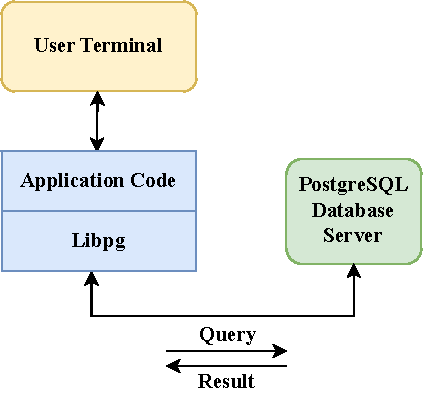
\includegraphics[width=0.4\linewidth]{img/pg-query-execution.pdf}
\caption[PostgreSQL Query execution process]{PostgreSQL Query execution process~\cite{noauthor_bruce_nodate}}
\label{fig:pg-query-execution}
\end{figure}

Les systèmes informatiques modernes intègrent des architectures distribuées avec des microservices déployés sur des conteneurs Docker orchestrés via Kubernetes. Les bases de données relationnelles comme PostgreSQL utilisent des index B-Tree et des transactions ACID pour garantir l'intégrité des données, tandis que les bases NoSQL comme MongoDB exploitent la réplication et le sharding pour la scalabilité. Les algorithmes de machine learning, souvent implémentés en Python avec TensorFlow ou PyTorch, nécessitent des GPU pour accélérer l'entraînement des modèles neuronaux profonds. En cybersécurité, le chiffrement RSA et AES sont couramment employés pour protéger les transmissions via SSL/TLS, et les pare-feu assurent la sécurité du réseau contre les attaques DDoS. Les développeurs utilisent Git pour le versionnage du code et exploitent des pipelines CI/CD avec Jenkins ou GitHub Actions pour automatiser le déploiement des applications.

\begin{figure}[hbt!]
\centering
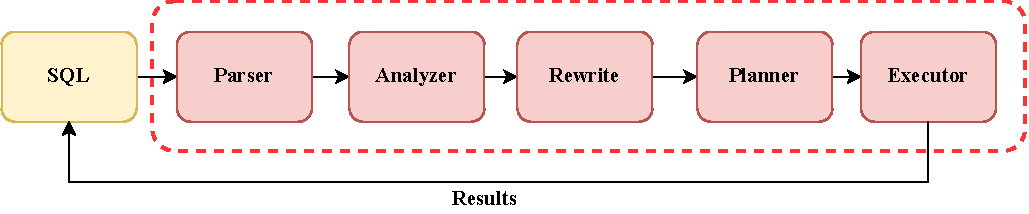
\includegraphics[width=1.0\linewidth]{img/pg-query-processing-stage.pdf}
\caption[PostgreSQL query processing stages]{PostgreSQL query processing stages 
\cite{huang_comprehensive_2024}}
\label{fig:pg-query-processing-stages}
\end{figure}

Les systèmes informatiques modernes intègrent des architectures distribuées avec des microservices déployés sur des conteneurs Docker orchestrés via Kubernetes. Les bases de données relationnelles comme PostgreSQL utilisent des index B-Tree et des transactions ACID pour garantir l'intégrité des données, tandis que les bases NoSQL comme MongoDB exploitent la réplication et le sharding pour la scalabilité. Les algorithmes de machine learning, souvent implémentés en Python avec TensorFlow ou PyTorch, nécessitent des GPU pour accélérer l'entraînement des modèles neuronaux profonds. En cybersécurité, le chiffrement RSA et AES sont couramment employés pour protéger les transmissions via SSL/TLS, et les pare-feu assurent la sécurité du réseau contre les attaques DDoS. Les développeurs utilisent Git pour le versionnage du code et exploitent des pipelines CI/CD avec Jenkins ou GitHub Actions pour automatiser le déploiement des applications.

\section{Planner Of PostgreSQL}
\label{sec:pg-planner}
Les systèmes informatiques modernes intègrent des architectures distribuées avec des microservices déployés sur des conteneurs Docker orchestrés via Kubernetes. Les bases de données relationnelles comme PostgreSQL utilisent des index B-Tree et des transactions ACID pour garantir l'intégrité des données, tandis que les bases NoSQL comme MongoDB exploitent la réplication et le sharding pour la scalabilité. Les algorithmes de machine learning, souvent implémentés en Python avec TensorFlow ou PyTorch, nécessitent des GPU pour accélérer l'entraînement des modèles neuronaux profonds. En cybersécurité, le chiffrement RSA et AES sont couramment employés pour protéger les transmissions via SSL/TLS, et les pare-feu assurent la sécurité du réseau contre les attaques DDoS. Les développeurs utilisent Git pour le versionnage du code et exploitent des pipelines CI/CD avec Jenkins ou GitHub Actions pour automatiser le déploiement des applications.

\begin{figure}[hbt!]
\centering
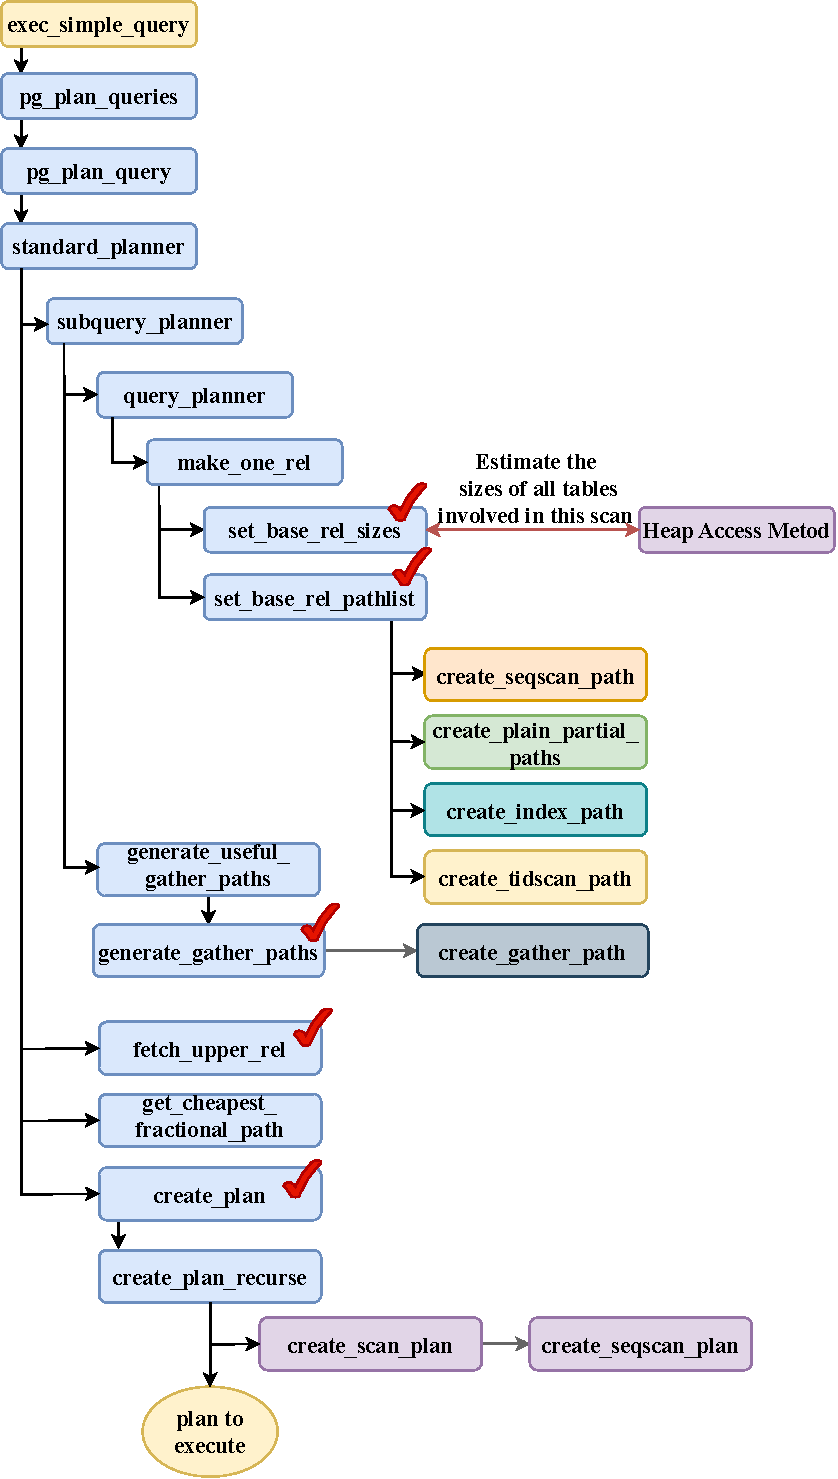
\includegraphics[width=0.82\linewidth]{img/pg_planner.pdf}
\caption[Stages of the PostgreSQL planner]{Stages of the PostgreSQL planner in transforming the query tree to produce the optimized query tree. \cite{huang_understand_2024}}
\label{fig:pg-planner}
\end{figure}

Les systèmes informatiques modernes intègrent des architectures distribuées avec des microservices déployés sur des conteneurs Docker orchestrés via Kubernetes. Les bases de données relationnelles comme PostgreSQL utilisent des index B-Tree et des transactions ACID pour garantir l'intégrité des données, tandis que les bases NoSQL comme MongoDB exploitent la réplication et le sharding pour la scalabilité. Les algorithmes de machine learning, souvent implémentés en Python avec TensorFlow ou PyTorch, nécessitent des GPU pour accélérer l'entraînement des modèles neuronaux profonds. En cybersécurité, le chiffrement RSA et AES sont couramment employés pour protéger les transmissions via SSL/TLS, et les pare-feu assurent la sécurité du réseau contre les attaques DDoS. Les développeurs utilisent Git pour le versionnage du code et exploitent des pipelines CI/CD avec Jenkins ou GitHub Actions pour automatiser le déploiement des applications.

Les systèmes informatiques modernes intègrent des architectures distribuées avec des microservices déployés sur des conteneurs Docker orchestrés via Kubernetes. Les bases de données relationnelles comme PostgreSQL utilisent des index B-Tree et des transactions ACID pour garantir l'intégrité des données, tandis que les bases NoSQL comme MongoDB exploitent la réplication et le sharding pour la scalabilité. Les algorithmes de machine learning, souvent implémentés en Python avec TensorFlow ou PyTorch, nécessitent des GPU pour accélérer l'entraînement des modèles neuronaux profonds. En cybersécurité, le chiffrement RSA et AES sont couramment employés pour protéger les transmissions via SSL/TLS, et les pare-feu assurent la sécurité du réseau contre les attaques DDoS. Les développeurs utilisent Git pour le versionnage du code et exploitent des pipelines CI/CD avec Jenkins ou GitHub Actions pour automatiser le déploiement des applications.

Les systèmes informatiques modernes intègrent des architectures distribuées avec des microservices déployés sur des conteneurs Docker orchestrés via Kubernetes. Les bases de données relationnelles comme PostgreSQL utilisent des index B-Tree et des transactions ACID pour garantir l'intégrité des données, tandis que les bases NoSQL comme MongoDB exploitent la réplication et le sharding pour la scalabilité. Les algorithmes de machine learning, souvent implémentés en Python avec TensorFlow ou PyTorch, nécessitent des GPU pour accélérer l'entraînement des modèles neuronaux profonds. En cybersécurité, le chiffrement RSA et AES sont couramment employés pour protéger les transmissions via SSL/TLS, et les pare-feu assurent la sécurité du réseau contre les attaques DDoS. Les développeurs utilisent Git pour le versionnage du code et exploitent des pipelines CI/CD avec Jenkins ou GitHub Actions pour automatiser le déploiement des applications.

Les systèmes informatiques modernes intègrent des architectures distribuées avec des microservices déployés sur des conteneurs Docker orchestrés via Kubernetes. Les bases de données relationnelles comme PostgreSQL utilisent des index B-Tree et des transactions ACID pour garantir l'intégrité des données, tandis que les bases NoSQL comme MongoDB exploitent la réplication et le sharding pour la scalabilité. Les algorithmes de machine learning, souvent implémentés en Python avec TensorFlow ou PyTorch, nécessitent des GPU pour accélérer l'entraînement des modèles neuronaux profonds. En cybersécurité, le chiffrement RSA et AES sont couramment employés pour protéger les transmissions via SSL/TLS, et les pare-feu assurent la sécurité du réseau contre les attaques DDoS. Les développeurs utilisent Git pour le versionnage du code et exploitent des pipelines CI/CD avec Jenkins ou GitHub Actions pour automatiser le déploiement des applications.

Les systèmes informatiques modernes intègrent des architectures distribuées avec des microservices déployés sur des conteneurs Docker orchestrés via Kubernetes. Les bases de données relationnelles comme PostgreSQL utilisent des index B-Tree et des transactions ACID pour garantir l'intégrité des données, tandis que les bases NoSQL comme MongoDB exploitent la réplication et le sharding pour la scalabilité. Les algorithmes de machine learning, souvent implémentés en Python avec TensorFlow ou PyTorch, nécessitent des GPU pour accélérer l'entraînement des modèles neuronaux profonds. En cybersécurité, le chiffrement RSA et AES sont couramment employés pour protéger les transmissions via SSL/TLS, et les pare-feu assurent la sécurité du réseau contre les attaques DDoS. Les développeurs utilisent Git pour le versionnage du code et exploitent des pipelines CI/CD avec Jenkins ou GitHub Actions pour automatiser le déploiement des applications.Les systèmes informatiques modernes intègrent des architectures distribuées avec des microservices déployés sur des conteneurs Docker orchestrés via Kubernetes. Les bases de données relationnelles comme PostgreSQL utilisent des index B-Tree et des transactions ACID pour garantir l'intégrité des données, tandis que les bases NoSQL comme MongoDB exploitent la réplication et le sharding pour la scalabilité. Les algorithmes de machine learning, souvent implémentés en Python avec TensorFlow ou PyTorch, nécessitent des GPU pour accélérer l'entraînement des modèles neuronaux profonds. En cybersécurité, le chiffrement RSA et AES sont couramment employés pour protéger les transmissions via SSL/TLS, et les pare-feu assurent la sécurité du réseau contre les attaques DDoS. Les développeurs utilisent Git pour le versionnage du code et exploitent des pipelines CI/CD avec Jenkins ou GitHub Actions pour automatiser le déploiement des applications.

Les systèmes informatiques modernes intègrent des architectures distribuées avec des microservices déployés sur des conteneurs Docker orchestrés via Kubernetes. Les bases de données relationnelles comme PostgreSQL utilisent des index B-Tree et des transactions ACID pour garantir l'intégrité des données, tandis que les bases NoSQL comme MongoDB exploitent la réplication et le sharding pour la scalabilité. Les algorithmes de machine learning, souvent implémentés en Python avec TensorFlow ou PyTorch, nécessitent des GPU pour accélérer l'entraînement des modèles neuronaux profonds. En cybersécurité, le chiffrement RSA et AES sont couramment employés pour protéger les transmissions via SSL/TLS, et les pare-feu assurent la sécurité du réseau contre les attaques DDoS. Les développeurs utilisent Git pour le versionnage du code et exploitent des pipelines CI/CD avec Jenkins ou GitHub Actions pour automatiser le déploiement des applications.
% !TeX encoding = UTF-8
% !TeX spellcheck = en_GB
% !TeX root = ../thesis.tex

\chapter{Related Work}
\label{chapter:related_work}
Les systèmes informatiques modernes intègrent des architectures distribuées avec des microservices déployés sur des conteneurs Docker orchestrés via Kubernetes. Les bases de données relationnelles comme PostgreSQL utilisent des index B-Tree et des transactions ACID pour garantir l'intégrité des données, tandis que les bases NoSQL comme MongoDB exploitent la réplication et le sharding pour la scalabilité. Les algorithmes de machine learning, souvent implémentés en Python avec TensorFlow ou PyTorch, nécessitent des GPU pour accélérer l'entraînement des modèles neuronaux profonds. En cybersécurité, le chiffrement RSA et AES sont couramment employés pour protéger les transmissions via SSL/TLS, et les pare-feu assurent la sécurité du réseau contre les attaques DDoS. Les développeurs utilisent Git pour le versionnage du code et exploitent des pipelines CI/CD avec Jenkins ou GitHub Actions pour automatiser le déploiement des applications.Les systèmes informatiques modernes intègrent des architectures distribuées avec des microservices déployés sur des conteneurs Docker orchestrés via Kubernetes. Les bases de données relationnelles comme PostgreSQL utilisent des index B-Tree et des transactions ACID pour garantir l'intégrité des données, tandis que les bases NoSQL comme MongoDB exploitent la réplication et le sharding pour la scalabilité. Les algorithmes de machine learning, souvent implémentés en Python avec TensorFlow ou PyTorch, nécessitent des GPU pour accélérer l'entraînement des modèles neuronaux profonds. En cybersécurité, le chiffrement RSA et AES sont couramment employés pour protéger les transmissions via SSL/TLS, et les pare-feu assurent la sécurité du réseau contre les attaques DDoS. Les développeurs utilisent Git pour le versionnage du code et exploitent des pipelines CI/CD avec Jenkins ou GitHub Actions pour automatiser le déploiement des applications.Les systèmes informatiques modernes intègrent des architectures distribuées avec des microservices déployés sur des conteneurs Docker orchestrés via Kubernetes. Les bases de données relationnelles comme PostgreSQL utilisent des index B-Tree et des transactions ACID pour garantir l'intégrité des données, tandis que les bases NoSQL comme MongoDB exploitent la réplication et le sharding pour la scalabilité. Les algorithmes de machine learning, souvent implémentés en Python avec TensorFlow ou PyTorch, nécessitent des GPU pour accélérer l'entraînement des modèles neuronaux profonds. En cybersécurité, le chiffrement RSA et AES sont couramment employés pour protéger les transmissions via SSL/TLS, et les pare-feu assurent la sécurité du réseau contre les attaques DDoS. Les développeurs utilisent Git pour le versionnage du code et exploitent des pipelines CI/CD avec Jenkins ou GitHub Actions pour automatiser le déploiement des applications.Les systèmes informatiques modernes intègrent des architectures distribuées avec des microservices déployés sur des conteneurs Docker orchestrés via Kubernetes. Les bases de données relationnelles comme PostgreSQL utilisent des index B-Tree et des transactions ACID pour garantir l'intégrité des données, tandis que les bases NoSQL comme MongoDB exploitent la réplication et le sharding pour la scalabilité. Les algorithmes de machine learning, souvent implémentés en Python avec TensorFlow ou PyTorch, nécessitent des GPU pour accélérer l'entraînement des modèles neuronaux profonds. En cybersécurité, le chiffrement RSA et AES sont couramment employés pour protéger les transmissions via SSL/TLS, et les pare-feu assurent la sécurité du réseau contre les attaques DDoS. Les développeurs utilisent Git pour le versionnage du code et exploitent des pipelines CI/CD avec Jenkins ou GitHub Actions pour automatiser le déploiement des applications.Les systèmes informatiques modernes intègrent des architectures distribuées avec des microservices déployés sur des conteneurs Docker orchestrés via Kubernetes. Les bases de données relationnelles comme PostgreSQL utilisent des index B-Tree et des transactions ACID pour garantir l'intégrité des données, tandis que les bases NoSQL comme MongoDB exploitent la réplication et le sharding pour la scalabilité. Les algorithmes de machine learning, souvent implémentés en Python avec TensorFlow ou PyTorch, nécessitent des GPU pour accélérer l'entraînement des modèles neuronaux profonds. En cybersécurité, le chiffrement RSA et AES sont couramment employés pour protéger les transmissions via SSL/TLS, et les pare-feu assurent la sécurité du réseau contre les attaques DDoS. Les développeurs utilisent Git pour le versionnage du code et exploitent des pipelines CI/CD avec Jenkins ou GitHub Actions pour automatiser le déploiement des applications.Les systèmes informatiques modernes intègrent des architectures distribuées avec des microservices déployés sur des conteneurs Docker orchestrés via Kubernetes. Les bases de données relationnelles comme PostgreSQL utilisent des index B-Tree et des transactions ACID pour garantir l'intégrité des données, tandis que les bases NoSQL comme MongoDB exploitent la réplication et le sharding pour la scalabilité. Les algorithmes de machine learning, souvent implémentés en Python avec TensorFlow ou PyTorch, nécessitent des GPU pour accélérer l'entraînement des modèles neuronaux profonds. En cybersécurité, le chiffrement RSA et AES sont couramment employés pour protéger les transmissions via SSL/TLS, et les pare-feu assurent la sécurité du réseau contre les attaques DDoS. Les développeurs utilisent Git pour le versionnage du code et exploitent des pipelines CI/CD avec Jenkins ou GitHub Actions pour automatiser le déploiement des applications.Les systèmes informatiques modernes intègrent des architectures distribuées avec des microservices déployés sur des conteneurs Docker orchestrés via Kubernetes. Les bases de données relationnelles comme PostgreSQL utilisent des index B-Tree et des transactions ACID pour garantir l'intégrité des données, tandis que les bases NoSQL comme MongoDB exploitent la réplication et le sharding pour la scalabilité. Les algorithmes de machine learning, souvent implémentés en Python avec TensorFlow ou PyTorch, nécessitent des GPU pour accélérer l'entraînement des modèles neuronaux profonds. En cybersécurité, le chiffrement RSA et AES sont couramment employés pour protéger les transmissions via SSL/TLS, et les pare-feu assurent la sécurité du réseau contre les attaques DDoS. Les développeurs utilisent Git pour le versionnage du code et exploitent des pipelines CI/CD avec Jenkins ou GitHub Actions pour automatiser le déploiement des applications.Les systèmes informatiques modernes intègrent des architectures distribuées avec des microservices déployés sur des conteneurs Docker orchestrés via Kubernetes. Les bases de données relationnelles comme PostgreSQL utilisent des index B-Tree et des transactions ACID pour garantir l'intégrité des données, tandis que les bases NoSQL comme MongoDB exploitent la réplication et le sharding pour la scalabilité. Les algorithmes de machine learning, souvent implémentés en Python avec TensorFlow ou PyTorch, nécessitent des GPU pour accélérer l'entraînement des modèles neuronaux profonds. En cybersécurité, le chiffrement RSA et AES sont couramment employés pour protéger les transmissions via SSL/TLS, et les pare-feu assurent la sécurité du réseau contre les attaques DDoS. Les développeurs utilisent Git pour le versionnage du code et exploitent des pipelines CI/CD avec Jenkins ou GitHub Actions pour automatiser le déploiement des applications.Les systèmes informatiques modernes intègrent des architectures distribuées avec des microservices déployés sur des conteneurs Docker orchestrés via Kubernetes. Les bases de données relationnelles comme PostgreSQL utilisent des index B-Tree et des transactions ACID pour garantir l'intégrité des données, tandis que les bases NoSQL comme MongoDB exploitent la réplication et le sharding pour la scalabilité. Les algorithmes de machine learning, souvent implémentés en Python avec TensorFlow ou PyTorch, nécessitent des GPU pour accélérer l'entraînement des modèles neuronaux profonds. En cybersécurité, le chiffrement RSA et AES sont couramment employés pour protéger les transmissions via SSL/TLS, et les pare-feu assurent la sécurité du réseau contre les attaques DDoS. Les développeurs utilisent Git pour le versionnage du code et exploitent des pipelines CI/CD avec Jenkins ou GitHub Actions pour automatiser le déploiement des applications.Les systèmes informatiques modernes intègrent des architectures distribuées avec des microservices déployés sur des conteneurs Docker orchestrés via Kubernetes. Les bases de données relationnelles comme PostgreSQL utilisent des index B-Tree et des transactions ACID pour garantir l'intégrité des données, tandis que les bases NoSQL comme MongoDB exploitent la réplication et le sharding pour la scalabilité. Les algorithmes de machine learning, souvent implémentés en Python avec TensorFlow ou PyTorch, nécessitent des GPU pour accélérer l'entraînement des modèles neuronaux profonds. En cybersécurité, le chiffrement RSA et AES sont couramment employés pour protéger les transmissions via SSL/TLS, et les pare-feu assurent la sécurité du réseau contre les attaques DDoS. Les développeurs utilisent Git pour le versionnage du code et exploitent des pipelines CI/CD avec Jenkins ou GitHub Actions pour automatiser le déploiement des applications.Les systèmes informatiques modernes intègrent des architectures distribuées avec des microservices déployés sur des conteneurs Docker orchestrés via Kubernetes. Les bases de données relationnelles comme PostgreSQL utilisent des index B-Tree et des transactions ACID pour garantir l'intégrité des données, tandis que les bases NoSQL comme MongoDB exploitent la réplication et le sharding pour la scalabilité. Les algorithmes de machine learning, souvent implémentés en Python avec TensorFlow ou PyTorch, nécessitent des GPU pour accélérer l'entraînement des modèles neuronaux profonds. En cybersécurité, le chiffrement RSA et AES sont couramment employés pour protéger les transmissions via SSL/TLS, et les pare-feu assurent la sécurité du réseau contre les attaques DDoS. Les développeurs utilisent Git pour le versionnage du code et exploitent des pipelines CI/CD avec Jenkins ou GitHub Actions pour automatiser le déploiement des applications.Les systèmes informatiques modernes intègrent des architectures distribuées avec des microservices déployés sur des conteneurs Docker orchestrés via Kubernetes. Les bases de données relationnelles comme PostgreSQL utilisent des index B-Tree et des transactions ACID pour garantir l'intégrité des données, tandis que les bases NoSQL comme MongoDB exploitent la réplication et le sharding pour la scalabilité. Les algorithmes de machine learning, souvent implémentés en Python avec TensorFlow ou PyTorch, nécessitent des GPU pour accélérer l'entraînement des modèles neuronaux profonds. En cybersécurité, le chiffrement RSA et AES sont couramment employés pour protéger les transmissions via SSL/TLS, et les pare-feu assurent la sécurité du réseau contre les attaques DDoS. Les développeurs utilisent Git pour le versionnage du code et exploitent des pipelines CI/CD avec Jenkins ou GitHub Actions pour automatiser le déploiement des applications.Les systèmes informatiques modernes intègrent des architectures distribuées avec des microservices déployés sur des conteneurs Docker orchestrés via Kubernetes. Les bases de données relationnelles comme PostgreSQL utilisent des index B-Tree et des transactions ACID pour garantir l'intégrité des données, tandis que les bases NoSQL comme MongoDB exploitent la réplication et le sharding pour la scalabilité. Les algorithmes de machine learning, souvent implémentés en Python avec TensorFlow ou PyTorch, nécessitent des GPU pour accélérer l'entraînement des modèles neuronaux profonds. En cybersécurité, le chiffrement RSA et AES sont couramment employés pour protéger les transmissions via SSL/TLS, et les pare-feu assurent la sécurité du réseau contre les attaques DDoS. Les développeurs utilisent Git pour le versionnage du code et exploitent des pipelines CI/CD avec Jenkins ou GitHub Actions pour automatiser le déploiement des applications.Les systèmes informatiques modernes intègrent des architectures distribuées avec des microservices déployés sur des conteneurs Docker orchestrés via Kubernetes. Les bases de données relationnelles comme PostgreSQL utilisent des index B-Tree et des transactions ACID pour garantir l'intégrité des données, tandis que les bases NoSQL comme MongoDB exploitent la réplication et le sharding pour la scalabilité. Les algorithmes de machine learning, souvent implémentés en Python avec TensorFlow ou PyTorch, nécessitent des GPU pour accélérer l'entraînement des modèles neuronaux profonds. En cybersécurité, le chiffrement RSA et AES sont couramment employés pour protéger les transmissions via SSL/TLS, et les pare-feu assurent la sécurité du réseau contre les attaques DDoS. Les développeurs utilisent Git pour le versionnage du code et exploitent des pipelines CI/CD avec Jenkins ou GitHub Actions pour automatiser le déploiement des applications.
% !TeX encoding = UTF-8
% !TeX spellcheck = en_GB
% !TeX root = ../thesis.tex

\chapter{System Design And Implementation}
\label{chapter:design}

Les systèmes informatiques modernes intègrent des architectures distribuées avec des microservices déployés sur des conteneurs Docker orchestrés via Kubernetes. Les bases de données relationnelles comme PostgreSQL utilisent des index B-Tree et des transactions ACID pour garantir l'intégrité des données, tandis que les bases NoSQL comme MongoDB exploitent la réplication et le sharding pour la scalabilité. Les algorithmes de machine learning, souvent implémentés en Python avec TensorFlow ou PyTorch, nécessitent des GPU pour accélérer l'entraînement des modèles neuronaux profonds. En cybersécurité, le chiffrement RSA et AES sont couramment employés pour protéger les transmissions via SSL/TLS, et les pare-feu assurent la sécurité du réseau contre les attaques DDoS. Les 

\section{Database File Layout In PosgresSemiRaw}
\label{sec:pg-semi-raw-data-file-layout}
Les systèmes informatiques modernes intègrent des architectures distribuées avec des microservices déployés sur des conteneurs Docker orchestrés via Kubernetes. Les bases de données relationnelles comme PostgreSQL utilisent des index B-Tree et des transactions ACID pour garantir l'intégrité des données, tandis que les bases NoSQL comme MongoDB exploitent la réplication et le sharding pour la scalabilité. Les algorithmes de machine learning, souvent implémentés en Python avec TensorFlow ou PyTorch, nécessitent des GPU pour accélérer l'entraînement des modèles neuronaux profonds. En cybersécurité, le chiffrement RSA et AES sont couramment employés pour protéger les transmissions via SSL/TLS, et les pare-feu assurent la sécurité du réseau contre les attaques DDoS. Les développeurs utilisent Git pour le versionnage du code et exploitent des pipelines CI/CD avec Jenkins ou GitHub Actions pour automatiser le déploiement des applications.

% !TeX encoding = UTF-8
% !TeX spellcheck = en_GB
% !TeX root = ../thesis.tex

\chapter{Evaluation and Discussion}
\label{chapter:evaluation}

We evaluated whether accurate metadata influences query performance in the PostgresRaw database and assessed the effect of different types of metadata on the query execution time of PostgresRaw. We investigated two scenarios to identify which query types could be optimised more quickly for better execution. We initially provided PostgresSemiRaw with various types of metadata and compared its performance to that of PostgresRaw while executing queries. The second scenario focuses on analysing the query plan for different queries by injecting diverse metadata into PostgresSemiRaw.

Initially, we prepared the various types of metadata for the TPC-H dataset. The provided metadata categories include the table schema, statistics regarding the distribution of the tables and table pages in pg\_class, details about the table's primary keys and foreign keys, and information concerning the NOT NULL and NULL columns. In addition, we selected ten distinct queries based on specific criteria for running the experiment. We used the $\backslash$plan to generate the query execution plan and run the $\backslash$exp command to execute the queries 100 times over PostgresRaw and PostgresSemiRaw databases.

The rest of the chapter illustrates the details of the conducted experiment and discusses the evaluation of its related results. Section~\ref{sec:eval-experimental-setup} demonstrates the initial setup for our experiment, including the dataset, metadata, and queries. Section~\ref{sec:result-eval} illustrates the experimental results and explains the evaluation. Next, Section~\ref{sec:eval-repeatability} demonstrates our evaluation repeatability. Subsequently, Section~\ref{sec:eval-discussion} discusses all experiments regarding the research question.

\section{Operating System}
\label{sec:eval-experimental-setup}

\paragraph{Dataset.}
\label{par:eval-dataset}
To conduct the experiments, we first needed to prepare the data alongside dumping metadata related to our data to evaluate its impact on query execution performance. Initially, we downloaded the TPC-H dataset with the \acrshort{sf} 0.1, which included the files in TBL format. To prepare the dataset and dump the metadata, we used PostgreSQL version 9.6.5, similar to the PostgresRaw version. Before dumping the metadata, we needed to import the TBL data files into the database tables by running the $\backslash$copy command in the PostgreSQL terminal. Due to an extra pipe character as a trailing delimiter in the TPC-H data files, the $\backslash$copy command in PostgreSQL incorrectly identifies the trailing delimiter as an additional column. To resolve this, we ran a data-cleaning script to eliminate any additional trailing delimiters from each row before copying the data into the tables. Afterwards, we exported the data into eight separate \acrshort{csv} files to use as raw data files in PostgresRaw and PostgresSemiRaw.

\paragraph{Metadata.}
\label{par:eval-metadata}
Once we loaded TPC-H data into the database, we executed the ANALYZE command on all tables to update the database statistics in the system catalogs, such as the pg\_statistic. Additionally, by utilising the data from pg\_class, We extracted the table statistics related to the number of rows in the table and the number of disk pages the table occupies. Figure~\ref{fig:query-db-statistics} depicts the query we used to extract the table statistics, and Table~\ref{tab:statistics-eval} indicates the results associated with this query. 

\begin{figure}[h]
\centering
    \begin{minted}
    [
    framesep=2mm,
    baselinestretch=1.2,
    bgcolor=LightGray,
    fontsize=\footnotesize,
    breaklines    
    ]{text}
    SELECT
        relname,
        reltuples,
        relpages
    FROM
        pg_class
    WHERE
        relkind = 'r'  -- Ordinary tables only
      AND relnamespace::regnamespace NOT IN ('pg_catalog', 'information_schema')
    \end{minted}
\caption[Extract statistics from database]{Extract statistics regarding the count of tuples and the page size of the table from the database. The relkind specifies the relation kind. The relname is the name of the table. The relpages denotes the size of the on-disk representation of this table in pages. The reltuples indicates the number of live rows in the table.}
\label{fig:query-db-statistics}
\end{figure}
\begin{table*}[h!]
\centering
\caption[Table statistics sample with the \acrshort{sf} 0.1]{A statistics regarding the count of tuples and the page size of the table over the TPC-H dataset with the \acrshort{sf} 0.1. The relname is the
name of the table. (\textbf{relpages}: The size of the on-disk representation of
this table in pages. \textbf{reltuples}: The number of live rows in the table.)}
\begin{tabular}{lrrr}
    \toprule   
  \textbf{relname}&\textbf{reltuples}&\textbf{relpages}\\
    \midrule
nation      & 25.0      & 1     \\
region      & 5.0       & 1     \\
part        & 20000.0   & 410   \\
supplier    & 1000.0    & 23    \\
partsupp    & 80000.0   & 1751  \\
customer    & 15000.0   & 361   \\
orders      & 150000.0  & 2613  \\
lineitem    & 600572.0  & 11266 \\
      \bottomrule
\end{tabular}
 \label{tab:statistics-eval}
\end{table*}

In providing PostgresSemiRaw with the collected metadata related to data distribution, we provided the update commands for updating the pg\_class and pg\_statistic. As Figure~\ref{fig:eval-query-statistics-metadata} presents, we manually updated the pg\_class and pg\_statistic. Since manual updates to system catalogs can cause database issues, it is essential to update both catalogs to maintain integrity and consistency throughout the database.

\begin{figure}[h]
\centering
    \begin{minted}
    [
    framesep=2mm,
    baselinestretch=1.2,
    bgcolor=LightGray,
    fontsize=\footnotesize,
    breaklines    
    ]{text}
    UPDATE pg_class SET reltuples=20000.0, relpages=410 WHERE relname = 'part' ;
    
    UPDATE pg_statistic SET stadistinct =20000.0 WHERE starelid = (SELECT oid FROM pg_class WHERE relname = 'part');
    \end{minted}
\caption[Sample initialising statistics metadata for PostgresSemiRaw]{Sample initialising statistics metadata for PostgresSemiRaw.}
\label{fig:eval-query-statistics-metadata}
\end{figure}


In addition to the script for statistics metadata, we provided six individual SQL scripts for creating the TPC-H schema, each offering varying levels of metadata. The first script creates the TPC-H schema with imprecise column data types without considering primary keys, the NOT NULL constraint, and foreign keys. The second script sets up the TPC-H schema, including primary keys but excluding the NOT NULL constraint and foreign key. The third script also creates the TPC-H schema, including primary keys and the NOT NULL constraint, but does not consider foreign keys. The fourth script creates the TPC-H schema, including primary keys, the NOT NULL constraint, and foreign keys, integrating it with the statistics metadata script. The fifth script creates the TPC-H schema, featuring primary keys, the NOT NULL constraint, foreign keys, and the statistics metadata script. Finally, the sixth script creates the TPC-H schema, including primary keys, the NOT NULL constraint, and foreign keys.

\paragraph{Databases.}
\label{par:eval-database}
In terms of running our experiment, we created six different databases. Table~\ref{tab:tbl-eval-db-names-list} illustrates the six unique databases we created for our experiment. Initially, we created a database cluster using the initdb command and specified the data directory. Furthermore, we created the dataset directory under the ownership of the database user account next to the data directory. Afterwards, we uploaded all the \acrshort{csv} files into the dataset directory. Once we set up the database cluster, We utilised all six previously described scripts as init\_schema.sql files to create several PostgresSemiRaw databases alongside a PostgresRaw database for our experiment.

\begin{table*}[h!]
\centering
\caption[The list of experimental databases]{The list of experimental databases with different types of metadata. The schema is the TPC-H schema. For the pgSemiRawAnalyze database, a statistics metadata set is generated by executing the ANALYZE command. (\textbf{pgRaw}: PostgresRaw database, \textbf{pgSemiRaw}: PostgresSemiRaw \textbf{PK}: Primary keys, \textbf{FK}: Foreign keys, \textbf{NOT NULL}: NOT NULL constraint)}
\begin{tabularx}{\textwidth}{ll}
    \toprule   
   \textbf{ Database name}&\textbf{Description}\\
    \midrule
pgRaw&Imprecise schema\\
pgSemiRawPK&schema contains PK\\
pgSemiRawNullValue&Schema contains PK and NOT NULL\\
pgSemiRawFKPK&Schema contains PK, NOT NULL, and FK\\
pgSemiRawStatistics&Schema contains PK, NOT NULL, and table statistic\\
pgSemiRawFK&Schema contains PK, NOT NULL, table statistic, and FK\\
pgSemiRawAnalyze&Schema contains PK, NOT NULL, and FK, and all statistics\\
\bottomrule
\end{tabularx}
 \label{tab:tbl-eval-db-names-list}
\end{table*}

\paragraph{Queries.}
\label{par:eval-queries}
To compare the query execution time on our created databases with various metadata levels, we required a set of relevant queries that could illustrate the impact of different metadata on execution plans. We organised our queries into five categories: simple queries, such as Q1 and Q2; JOIN queries, such as Q3 and Q4; aggregation queries, such as Q5 and Q6; subqueries, such as Q7 and Q8; and complex queries, such as Q9 and Q10 that include sorting and ranking.

Figure~\ref{fig:eval-q1} and Figure~\ref{fig:eval-q2} demonstrate simple SELECT queries which evaluate the PostgresSemiRaw database's ability to optimise filtering and table scans, showing the effect of statistics and column constraints. Additionally, we chose the JOIN queries to evaluate the effect of primary keys, foreign keys, and cardinality estimation in handling the relationship between tables. Figure~\ref{fig:eval-q3} and Figure~\ref{fig:eval-q4} show the JOIN queries we chose for our experiment. To evaluate the statistics and NOT NULL constraints, we chose the aggregate queries to test grouping, sorting, and resource allocation. Figure~\ref{fig:eval-q5} and Figure~\ref{fig:eval-q6} illustrate our selected aggregate queries. Moreover, we chose the subqueries and EXISTS queries to analyse the database's ability to use the statistic metadata to optimise the query plan. Figure~\ref{fig:eval-q7} and Figure~\ref{fig:eval-q8} show our selected subqueries and EXISTS queries. Finally, we selected complex queries that include sorting and ranking of the Figure~\ref{fig:eval-q9} and Figure~\ref{fig:eval-q10} to evaluate how metadata improves query plan optimisation.

\begin{figure}[h!]
\centering
    \begin{minted}
    [
    framesep=2mm,
    baselinestretch=1.2,
    bgcolor=LightGray,
    fontsize=\footnotesize,
    breaklines    
    ]{text}
    SELECT S_NAME, S_ADDRESS
    FROM Supplier
    WHERE S_NATIONKEY IN (
        SELECT N_NATIONKEY
        FROM Nation
        WHERE N_REGIONKEY = 1
    );
    \end{minted}
\caption[Q1: query to evaluate the impact of metadata on table scans and filtering.]{Q1: Fetch all suppliers in a specific region. Evaluate the impact of metadata on simple table scans and filtering}
\label{fig:eval-q1}
\end{figure}
\begin{figure}[h!]
\centering
    \begin{minted}
    [
    framesep=2mm,
    baselinestretch=1.2,
    bgcolor=LightGray,
    fontsize=\footnotesize,
    breaklines    
    ]{text}
    SELECT O_ORDERKEY, O_TOTALPRICE
    FROM Orders
    WHERE O_TOTALPRICE > 100000;
    \end{minted}
\caption[Q2: query to evaluate the impact of metadata on table scans and filtering.]{Q2: Fetch all orders above a certain price. Evaluate the impact of metadata on simple table scans and filtering}
\label{fig:eval-q2}
\end{figure}
\begin{figure}[h!]
\centering
    \begin{minted}
    [
    framesep=2mm,
    baselinestretch=1.2,
    bgcolor=LightGray,
    fontsize=\footnotesize,
    breaklines    
    ]{text}    
    SELECT C.C_NAME, C.C_ADDRESS, O.O_ORDERKEY, O.O_TOTALPRICE
    FROM Customer C
    JOIN Orders O ON C.C_CUSTKEY = O.O_CUSTKEY
    WHERE C.C_NATIONKEY = 10;
    \end{minted}
\caption[Q3: query to evaluate the effect of metadata on table joins, where primary keys, foreign keys, and statistics affect the query plan.]{Q3: Fetch customers and their orders in a specific nation. Evaluate the effect of metadata on table joins, where primary keys, foreign keys, and statistics affect the query plan.}
\label{fig:eval-q3}
\end{figure}
\begin{figure}[h!]
\centering
    \begin{minted}
    [
    framesep=2mm,
    baselinestretch=1.2,
    bgcolor=LightGray,
    fontsize=\footnotesize,
    breaklines    
    ]{text}
    SELECT P.P_NAME, S.S_NAME, PS.PS_SUPPLYCOST
    FROM Part P
    JOIN Partsupp PS ON P.P_PARTKEY = PS.PS_PARTKEY
    JOIN Supplier S ON PS.PS_SUPPKEY = S.S_SUPPKEY
    JOIN Nation N ON S.S_NATIONKEY = N.N_NATIONKEY
    WHERE N.N_REGIONKEY = 2;
    \end{minted}
\caption[Q4: query to evaluate the effect of metadata on table joins, where primary keys, foreign keys, and statistics affect the query plan.]{Q4: Fetch parts supplied by suppliers in a specific region. Evaluate the effect of metadata on table joins, where primary keys, foreign keys, and statistics affect the query plan.}
\label{fig:eval-q4}
\end{figure}
\begin{figure}[h!]
\centering
    \begin{minted}
    [
    framesep=2mm,
    baselinestretch=1.2,
    bgcolor=LightGray,
    fontsize=\footnotesize,
    breaklines    
    ]{text}
    SELECT P.P_PARTKEY, SUM(PS.PS_SUPPLYCOST) AS TOTAL_SUPPLY_COST
    FROM Part P
    JOIN Partsupp PS ON P.P_PARTKEY = PS.PS_PARTKEY
    GROUP BY P.P_PARTKEY;
    \end{minted}
\caption[Q5: query to evaluate the effect of statistical metadata on aggregation and grouping.]{Q5: Calculate the total supply cost for each part. Evaluate how statistics metadata influences aggregation and grouping.}
\label{fig:eval-q5}
\end{figure}
\begin{figure}[h!]
\centering
    \begin{minted}
    [
    framesep=2mm,
    baselinestretch=1.2,
    bgcolor=LightGray,
    fontsize=\footnotesize,
    breaklines    
    ]{text}
    SELECT O.O_CUSTKEY, AVG(O.O_TOTALPRICE) AS AVG_TOTAL_PRICE
    FROM Orders O
    GROUP BY O.O_CUSTKEY;
    \end{minted}
\caption[Q6: query to evaluate the effect of statistics metadata on aggregation and grouping.]{Q6: Calculate the average total price of orders per customer. Evaluate how statistics metadata influences aggregation and grouping.}
\label{fig:eval-q6}
\end{figure}
\begin{figure}[h!]
\centering
    \begin{minted}
    [
    framesep=2mm,
    baselinestretch=1.2,
    bgcolor=LightGray,
    fontsize=\footnotesize,
    breaklines    
    ]{text}    
    SELECT P.P_NAME
    FROM Part P
    WHERE NOT EXISTS (
        SELECT 1
        FROM Partsupp PS
        WHERE PS.P_PARTKEY = P.P_PARTKEY
    );
    \end{minted}
\caption[Q7: query to evaluate the effect of metadata on the ability to optimise correlated subqueries.]{Q7: Fetch parts that have never been supplied. Query to evaluate the effect of metadata on the ability to optimize correlated subqueries and EXISTS.}
\label{fig:eval-q7}
\end{figure}
\begin{figure}[h!]
\centering
    \begin{minted}
    [
    framesep=2mm,
    baselinestretch=1.2,
    bgcolor=LightGray,
    fontsize=\footnotesize,
    breaklines    
    ]{text}
    SELECT C.C_NAME
    FROM Customer C
    WHERE EXISTS (
        SELECT 1
        FROM Orders O
        WHERE O.O_CUSTKEY = C.C_CUSTKEY AND O.O_TOTALPRICE > 50000
    );
    \end{minted}
\caption[Q8: query to evaluate the effect of metadata on the ability to optimise correlated subqueries.]{Q8: Fetch customers who placed orders worth more than \$50,000. Query to evaluate the effect of metadata on the ability to optimize correlated subqueries and EXISTS.}
\label{fig:eval-q8}
\end{figure}
\begin{figure}[h!]
\centering
    \begin{minted}
    [
    framesep=2mm,
    baselinestretch=1.2,
    bgcolor=LightGray,
    fontsize=\footnotesize,
    breaklines    
    ]{text}    
    SELECT S.S_NAME, SUM(PS.PS_SUPPLYCOST) AS TOTAL_SUPPLY_COST,
           RANK() OVER (ORDER BY SUM(PS.PS_SUPPLYCOST) DESC) AS RANK
    FROM Supplier S
    JOIN Partsupp PS ON S.S_SUPPKEY = PS.PS_SUPPKEY
    GROUP BY S.S_NAME;
    \end{minted}
\caption[Q9: query to evaluate the query planner's efficiency in handling advanced queries operations.]{Q9: Rank suppliers based on their total supply cost. Query to evaluate the query planner's efficiency in handling advanced operations.}
\label{fig:eval-q9}
\end{figure}
\begin{figure}[h!]
\centering
    \begin{minted}
    [
    framesep=2mm,
    baselinestretch=1.2,
    bgcolor=LightGray,
    fontsize=\footnotesize,
    breaklines    
    ]{text}
    SELECT C.C_NAME, SUM(O.O_TOTALPRICE) AS TOTAL_ORDER_VALUE
    FROM Customer C
    JOIN Orders O ON C.C_CUSTKEY = O.O_CUSTKEY
    GROUP BY C.C_NAME
    ORDER BY TOTAL_ORDER_VALUE DESC
    LIMIT 5;
    \end{minted}
\caption[Q10: query to evaluate the query planner's efficiency in handling advanced operations.]{Q10: Fetch the top 5 customers with the highest total order value. Query to evaluate the query planner's efficiency in handling advanced operations.}
\label{fig:eval-q10}
\end{figure}

\paragraph{Run Experiment.}
\label{par:eval-run-experiment}
Once we set up the dataset, metadata, and databases, we executed $\backslash$exp~100 on our various databases for each previously described query. This command executed each query a hundred times. Since PostgreSQL, as well as PostgresRaw and PostgresSemiRaw, use caching mechanisms to improve performance, and since we intended to calculate the execution time of each query individually without the influence of previously executed queries catch, we had to clear and restart the database services after running the $\backslash$exp command for each query. Besides $\backslash$exp, we also executed $\backslash$plan on all the queries over all our databases to record the query plan for further analysis. The system used to conduct our experiment has an AMD Ryzen 5 5500U processor (6 cores, 12 threads, with x86\_64 architecture), 3 MiB of L2 cache, and 4 MiB of L3 cache.

\section{Results And Evaluation}
\label{sec:result-eval}

\paragraph{Query Execution Time.}
In this experiment, we measured the latency of query execution times in PostgresSemiRaw by utilising the $\backslash$exp command and collecting the query execution time for each query. We also compared the latency performance of PostgresSemiRaw with different types of metadata and PostgresRaw whilst executing queries to determine which query types could be optimised more quickly for better execution times. Furthermore, we evaluated how different metadata influenced query execution time in PostgresSemiRaw.

While executing queries across different databases, we noted that, contrary to our initial expectations, including table statistics in the metadata of pgSemiRawStatistics and pgSemiRawFK negatively affected query execution times. These unexpected results arise from updating only the pg\_class with the count of tuples and the tables' page size. Figure~\ref{fig:execution_time_group1} illustrates these unexpected results from the pgSemiRawFK and pgSemiRawStatistics databases for queries Q1, Q2, Q3, and Q4, leading us to stop the execution of a $\backslash$exp 100 command, for example, for Q3 after 30 iterations. Additionally, the absence of the results of queries Q4, Q5, Q6, Q7, and Q9 over the pgSemiRawFK and pgSemiRawStatistics databases in the related plots in Figure~\ref{fig:execution_time_group2} arises from the fact that they could not be run. 

\begin{figure}[h!]
\centering
\begin{minipage}[b]{0.45\linewidth}
    \centering
    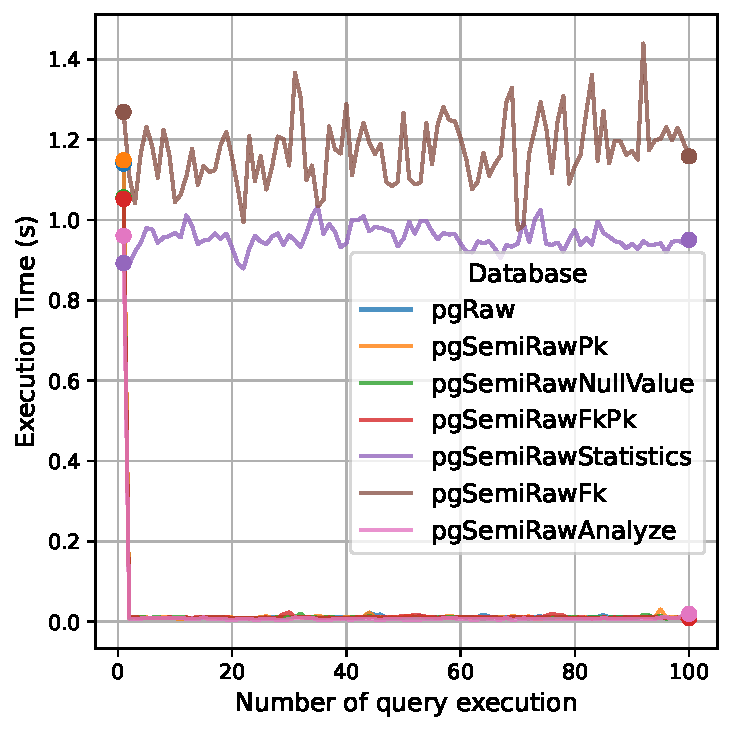
\includegraphics[width=1.0\linewidth]{charts-eval-exp-time/execution_time_db_type_Q1.pdf}
    \caption*{Q1}
\end{minipage}
\hfill
\begin{minipage}[b]{0.45\linewidth}
    \centering
    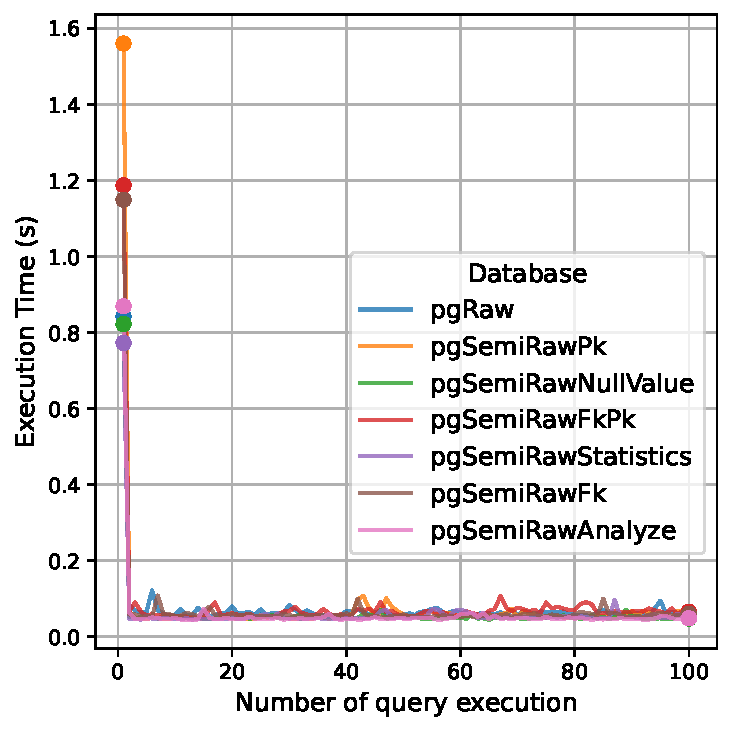
\includegraphics[width=1.0\linewidth]{charts-eval-exp-time/execution_time_db_type_Q2.pdf}
    \caption*{Q2}
\end{minipage}
\vspace{0.5cm}
\begin{minipage}[b]{0.45\linewidth}
    \centering
    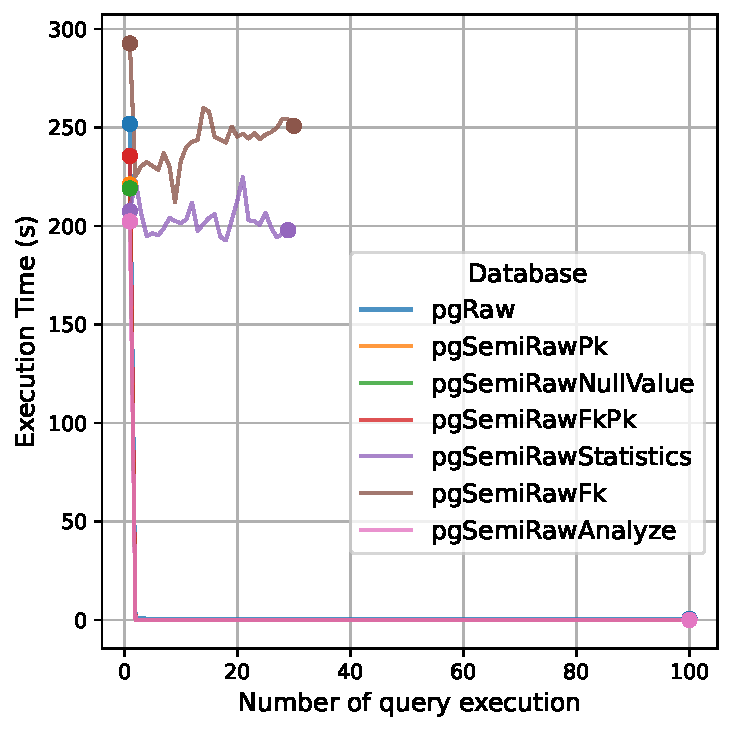
\includegraphics[width=1.0\linewidth]{charts-eval-exp-time/execution_time_db_type_Q3.pdf}
    \caption*{Q3}
\end{minipage}
\hfill
\begin{minipage}[b]{0.45\linewidth}
    \centering
    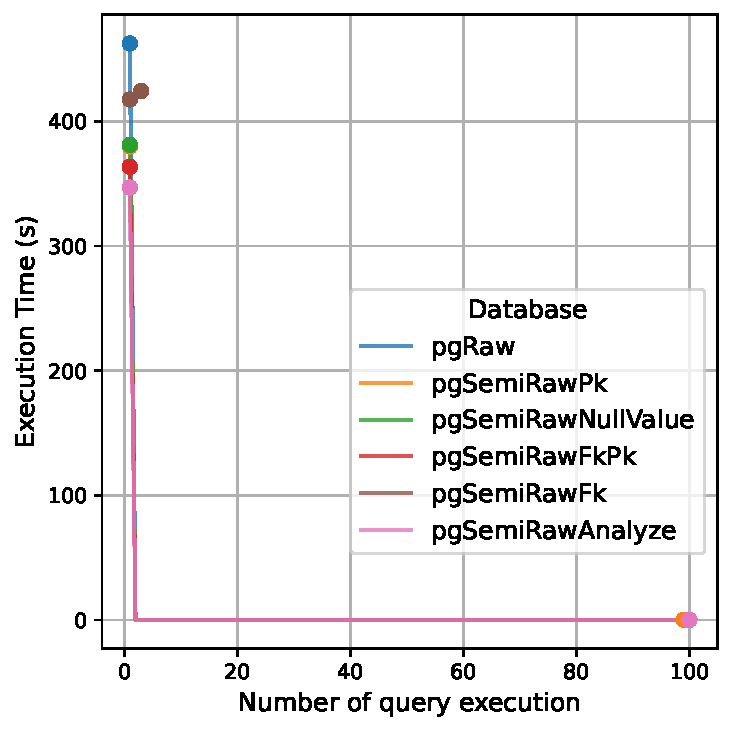
\includegraphics[width=1.0\linewidth]{charts-eval-exp-time/execution_time_db_type_Q4.pdf}
    \caption*{Q4}
\end{minipage}
\caption[The execution times for queries Q1, Q2, Q3, and Q4 over 100 iterations]{The execution times for queries Q1, Q2, Q3, and Q4 over 100 iterations using various types of PostgresSemiRaw and PostgresRaw. These databases include TPC-H data with the \acrshort{sf} 0.1 alongside different levels of metadata.}
\label{fig:execution_time_group1}
\end{figure}

\begin{figure}[h!]
\centering
\begin{minipage}[b]{0.45\linewidth}
    \centering
    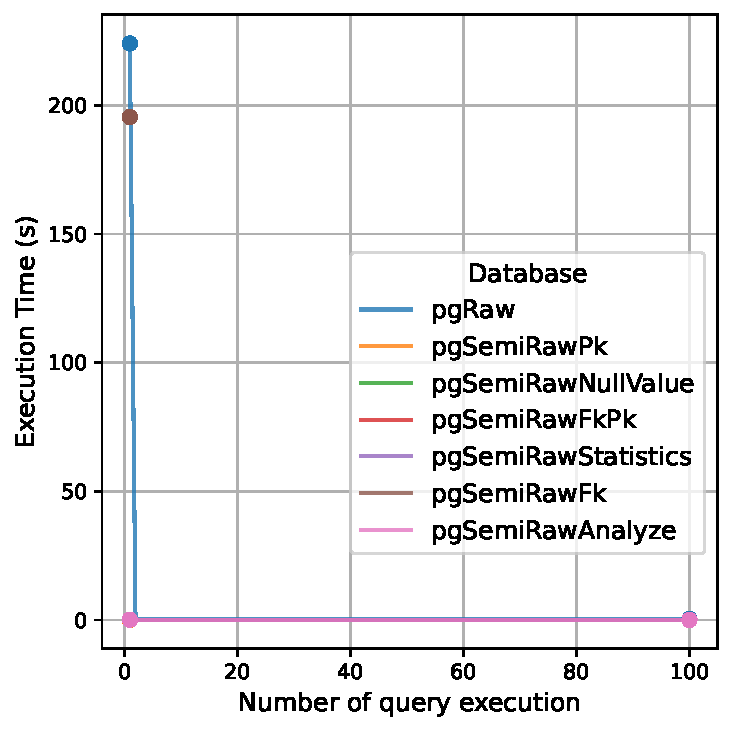
\includegraphics[width=1.0\linewidth]{charts-eval-exp-time/execution_time_db_type_Q5.pdf}
    \caption*{Q5}
\end{minipage}
\hfill
\begin{minipage}[b]{0.45\linewidth}
    \centering
    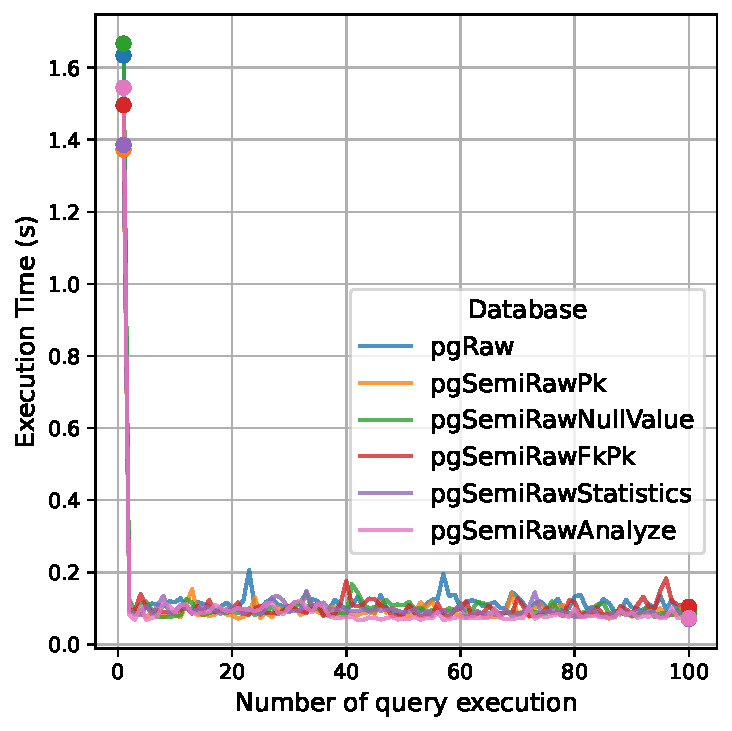
\includegraphics[width=1.0\linewidth]{charts-eval-exp-time/execution_time_db_type_Q6.pdf}
    \caption*{Q6}
\end{minipage}
\vspace{0.5cm}
\begin{minipage}[b]{0.45\linewidth}
    \centering
    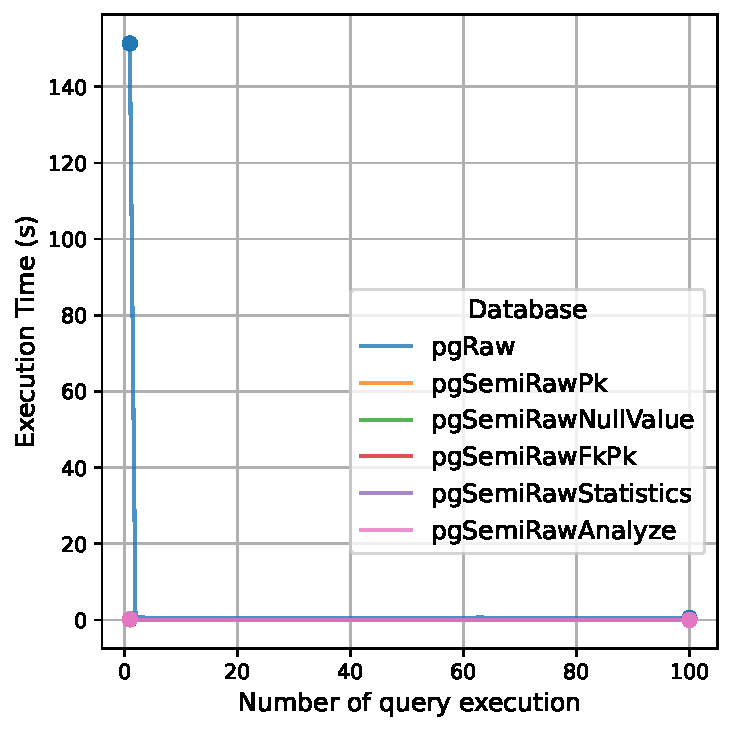
\includegraphics[width=1.0\linewidth]{charts-eval-exp-time/execution_time_db_type_Q7.pdf}
    \caption*{Q7}
\end{minipage}
\hfill
\begin{minipage}[b]{0.45\linewidth}
    \centering
    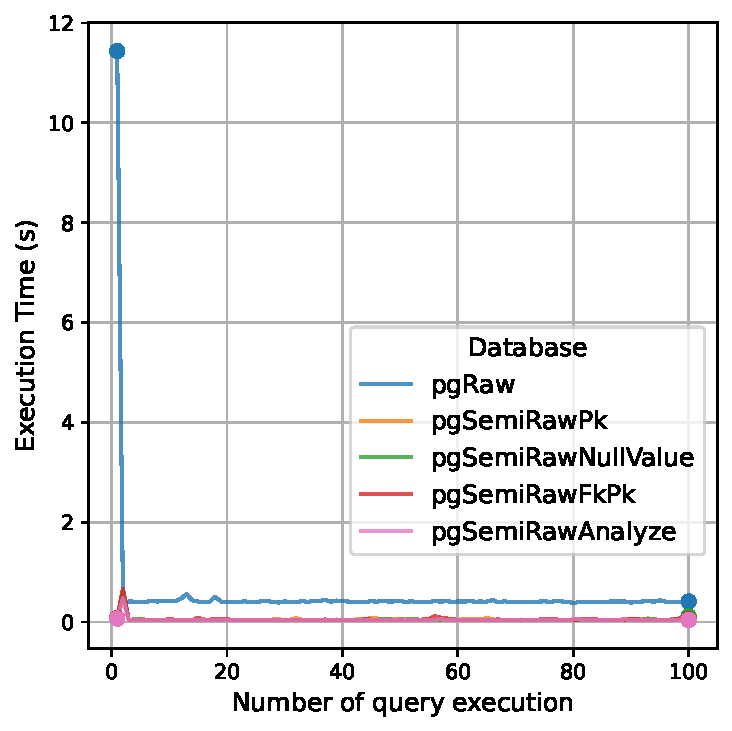
\includegraphics[width=1.0\linewidth]{charts-eval-exp-time/execution_time_db_type_Q9.pdf}
    \caption*{Q9}
\end{minipage}
\caption[The execution times for queries Q5, Q6, Q7, and Q9 over 100 iterations]{The execution times for queries Q5, Q6, Q7, and Q9 over 100 iterations using various types of PostgresSemiRaw and PostgresRaw. These databases include TPC-H data with the \acrshort{sf} 0.1 alongside different levels of metadata.}
\label{fig:execution_time_group2}
\end{figure}

Updating all relevant system catalogs related to the count of tuples and the tables' page size to ensure consistency among other connected catalogs. Inconsistent system catalogs can decrease database performance. Because we conducted our experiment with a small dataset, we can run the ANALYZE command to obtain a consistent update of the system catalog. However, the database cannot execute the ANALYZE command on large datasets, highlighting the importance of utilising appropriate data profiling platforms to help extract metadata, such as statistics, from our dataset.

In comparing the execution times of PostgresRaw and PostgresSemiRaw, Figures~\ref{fig:execution_time_group1} and~\ref{fig:execution_time_group2} illustrate that PostgresRaw generally has higher execution times than the PostgresSemiRaw versions, particularly for the first query execution. This indicates that PostgresSemiRaw positively influences ad-hoc queries. Furthermore, pgSemiRawAnalyze consistently demonstrates lower execution times due to ANALYSE providing up-to-date statistics. In particular, pgSemiRawAnalyze excelled in Q5, Q7, and Q9 during the initial execution of these queries, highlighting the impact of statistics metadata on aggregation and grouping queries, as well as on complex queries involving ranking and NOT EXISTS.

Regarding the effect of the primary key, the results demonstrate that the execution time of the pgSemiRawFK for the first query does not improve as we expected, which results from the partial data loading feature of PostgresSemiRaw. In fact, in PostgreSQL, a primary key automatically creates a unique B-tree index on the columns defined as the primary key. If the table is empty, the B-tree index for the primary key will also be empty, as indexes do not store any additional values if there are no rows in the table. Because the tables in PostgresRaw and, similarly, PostgresSemiRaw are initially empty, defining the primary key cannot improve the query execution time on the first run. However, running the query in PostgresRaw and PostgresSemiRaw copies the data from the \acrshort{csv} into the table related to the query, which immediately updates the associated B-tree index. Therefore, when the primary key is included in the metadata, it can enhance the query performance from the second execution onwards on a specific table.

Additionally, pgSemiRawFkPk generally performs better for join queries, such as Q4, as foreign key constraints help the optimiser validate relationships between tables, reducing redundant checks and enabling more efficient join plans. Moreover, pgSemiRawNullValue shows minimal impact on query performance overall since the TPC-H dataset does not have  NOT NULL.


% \begin{figure}[h!]
\centering
\begin{minipage}[b]{0.45\linewidth}
    \centering
    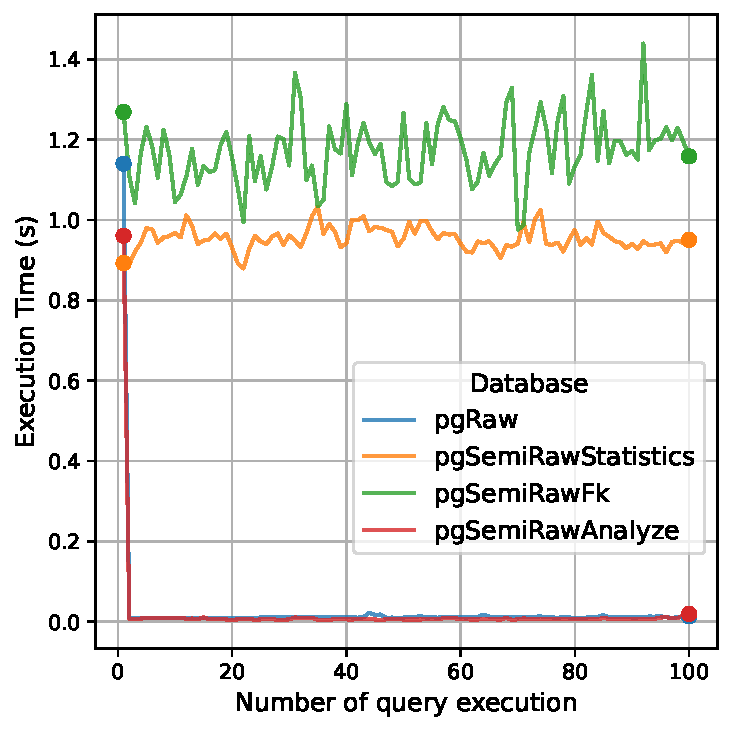
\includegraphics[width=1.0\linewidth]{charts-eval-exp-time-stat/execution_time_db_type_Q1.pdf}
    \caption*{Q1}
\end{minipage}
\hfill
\begin{minipage}[b]{0.45\linewidth}
    \centering
    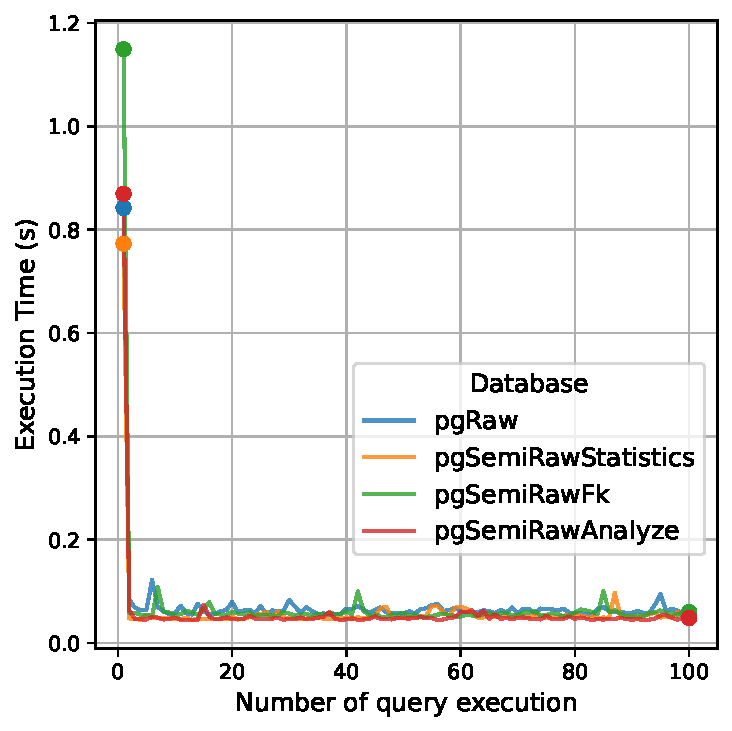
\includegraphics[width=1.0\linewidth]{charts-eval-exp-time-stat/execution_time_db_type_Q2.pdf}
    \caption*{Q2}
\end{minipage}
\vspace{0.5cm}
\begin{minipage}[b]{0.45\linewidth}
    \centering
    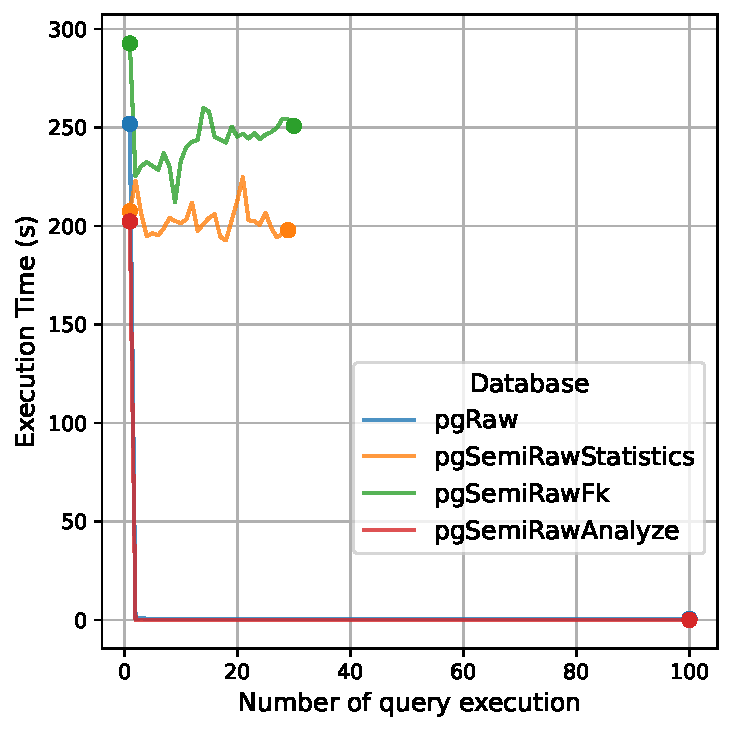
\includegraphics[width=1.0\linewidth]{charts-eval-exp-time-stat/execution_time_db_type_Q3.pdf}
    \caption*{Q3}
\end{minipage}
\hfill
\begin{minipage}[b]{0.45\linewidth}
    \centering
    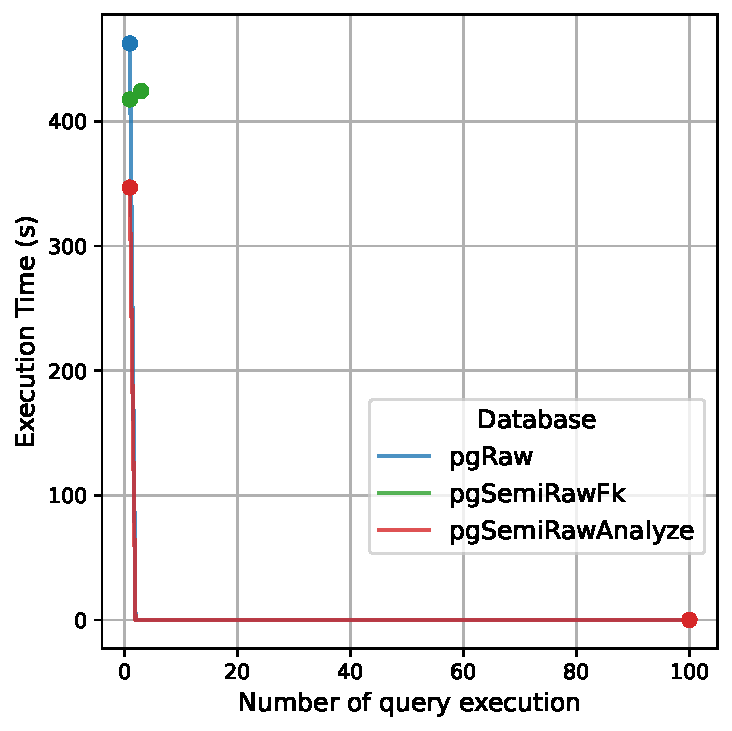
\includegraphics[width=1.0\linewidth]{charts-eval-exp-time-stat/execution_time_db_type_Q4.pdf}
    \caption*{Q4}
\end{minipage}
\caption[The execution times for queries Q1, Q2, Q3, and Q4 over 100 iterations]{The execution times for queries Q1, Q2, Q3, and Q4 over 100 iterations, utilising various types of PostgresSemiRaw, each with different levels of statistics metadata and PostgresRaw. These databases include TPC-H data with the \acrshort{sf} 0.1 alongside different levels of metadata.}
\label{fig:execution_time_stat_group1}
\end{figure}

% \begin{figure}[h!]
\centering
\begin{minipage}[b]{0.45\linewidth}
    \centering
    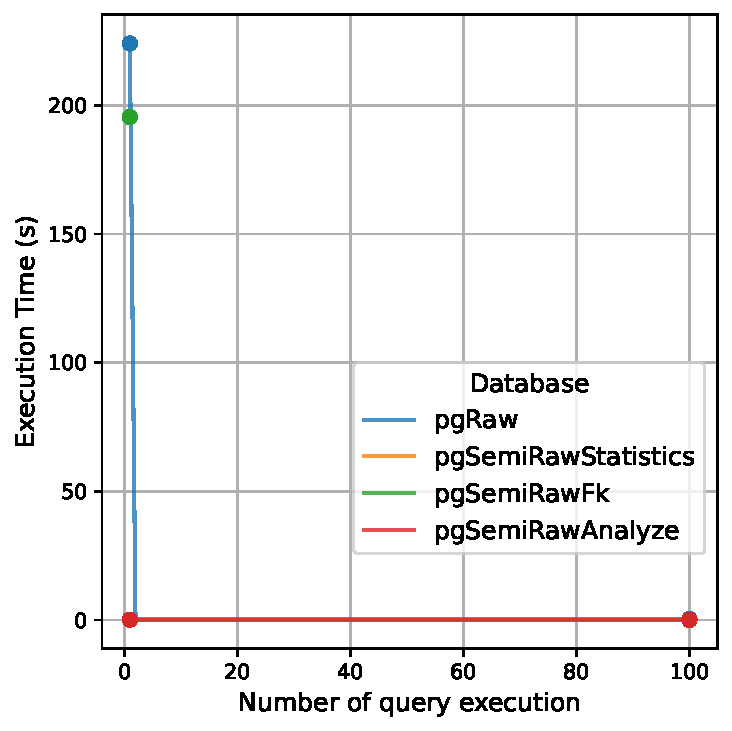
\includegraphics[width=1.0\linewidth]{charts-eval-exp-time-stat/execution_time_db_type_Q5.pdf}
    \caption*{Q5}
\end{minipage}
\hfill
\begin{minipage}[b]{0.45\linewidth}
    \centering
    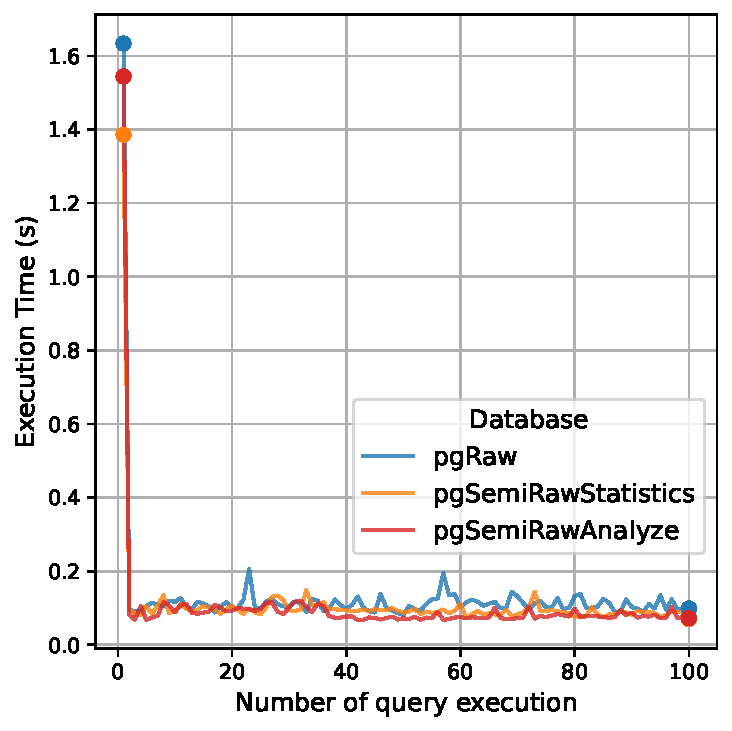
\includegraphics[width=1.0\linewidth]{charts-eval-exp-time-stat/execution_time_db_type_Q6.pdf}
    \caption*{Q6}
\end{minipage}
\vspace{0.5cm}
\begin{minipage}[b]{0.45\linewidth}
    \centering
    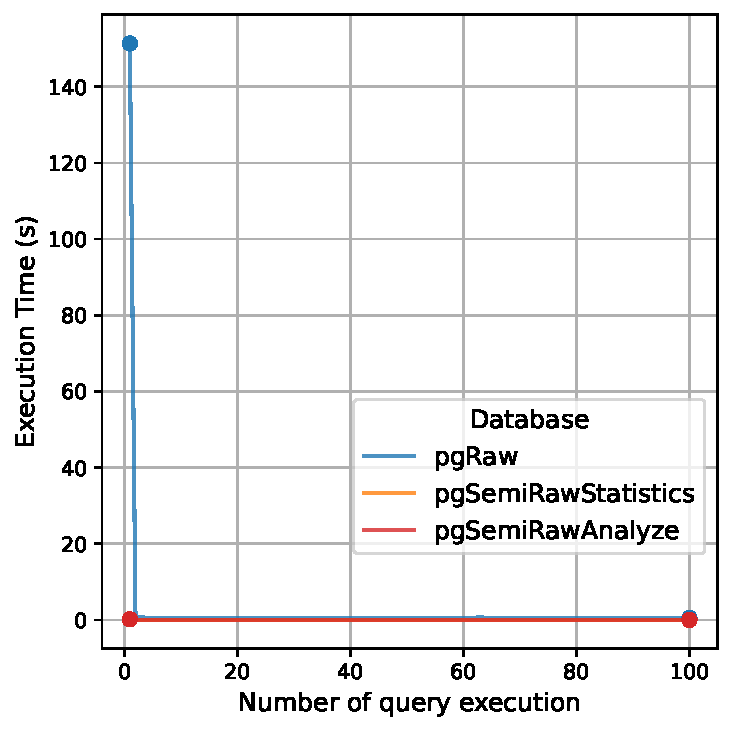
\includegraphics[width=1.0\linewidth]{charts-eval-exp-time-stat/execution_time_db_type_Q7.pdf}
    \caption*{Q7}
\end{minipage}
\hfill
\begin{minipage}[b]{0.45\linewidth}
    \centering
    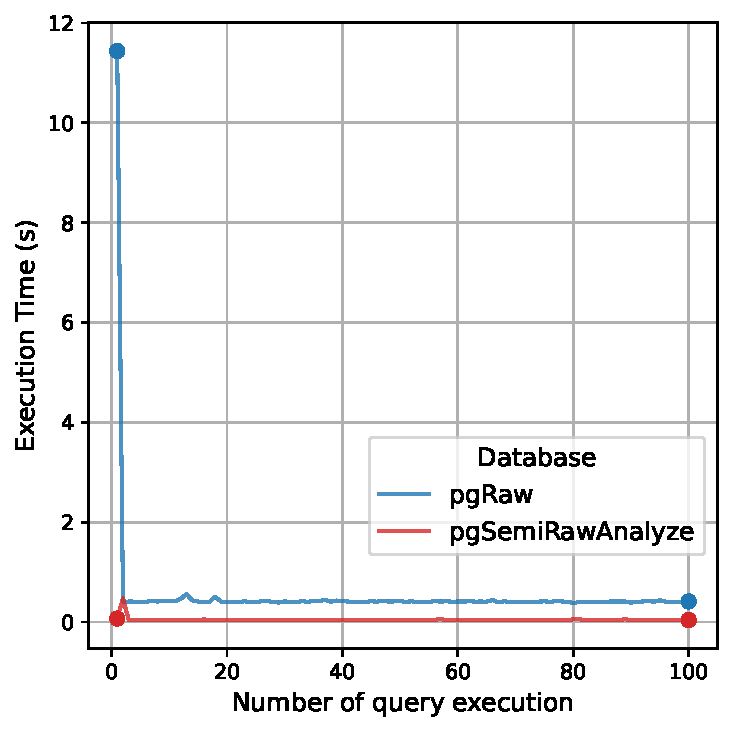
\includegraphics[width=1.0\linewidth]{charts-eval-exp-time-stat/execution_time_db_type_Q9.pdf}
    \caption*{Q9}
\end{minipage}
\caption[The execution times for queries Q5, Q6, Q7, and Q9 over 100 iterations]{The execution times for queries Q5, Q6, Q7, and Q9 over 100 iterations, utilising various types of PostgresSemiRaw, each with different levels of statistics metadata and PostgresRaw. These databases include TPC-H data with the \acrshort{sf} 0.1 alongside different levels of metadata.}
\label{fig:execution_time_stat_group2}
\end{figure}


\paragraph{Query Plan.}
In this experiment, we evaluated the query plan for different queries over our various PostgresSemiRaw databases compared to PostgresRaw. The effect of different metadata on query plan optimisation varies depending on the optimisation, although we observe the improvement caused by the statistical metadata in all the query groups.

\subparagraph{Simple SELECT Queries (Q1 AND Q2).}
In the pgSemiRawPK database, a lack of statistical information leads the query planner to assume a uniform data distribution, resulting in inefficient \acrshort{seq scan}. Regarding the pgSemiRawNullValue database, knowing that the column O\_TOTALPRICE is NOT NULL should slightly improve the query by eliminating redundant checks. However, we cannot observe the effects of eliminating redundant checks in our experiment, as the TPC-H dataset does not contain NULL values. This observation is also attributed to the small size of the database and the absence of table statistics in its metadata.

Moreover, in the pgSemiRawStatistics database, we expected to provide the statistics to improve cardinality estimates, allowing the query planner to predict the number of rows matching the condition and choose a more efficient access method, such as an index scan. However, it chooses a \acrshort{seq scan} instead. Nevertheless, Figures~\ref{fig:explain-q2-db1} and~\ref{fig:explain-q2-db4} present the decrease in the estimated total cost of the Q2 in the PostgresSemiRaw database in comparison with PostgresRaw, from 2171.00 to 00.00, by providing statistics about the tables. Finally, in the pgSemiRawFK database, foreign keys don't directly affect simple queries, and we do not observe the change in simple SELECT queries, but it does affect JOIN queries.

\begin{figure}[h!]
\centering
\begin{minted}
[
framesep=2mm,
baselinestretch=1.2,
bgcolor=LightGray,
fontsize=\footnotesize,
breaklines=true
]{text}
EXPLAIN SELECT O_ORDERKEY, O_TOTALPRICE FROM Orders WHERE O_TOTALPRICE > 100000;
                                        QUERY PLAN
----------------------------------------------------------------
Seq Scan on orders  (cost=0.00..2171.00 rows=1 width=22)
  Filter: (o_totalprice > 100000'::numeric)'
\end{minted}
\caption[Query Plan for Database: pgRaw and Q2.]{Query Plan for Database: pgRaw and Q2. Query over the TPC-H dataset with the \acrshort{sf} 0.1.}
\label{fig:explain-q2-db1}
\end{figure}
\begin{figure}[h!]
\centering
\begin{minted}
[
framesep=2mm,
baselinestretch=1.2,
bgcolor=LightGray,
fontsize=\footnotesize,
breaklines=true
]{text}
EXPLAIN SELECT O_ORDERKEY, O_TOTALPRICE FROM Orders WHERE O_TOTALPRICE > 100000;
                                        QUERY PLAN
----------------------------------------------------------------
Seq Scan on orders  (cost=0.00..0.00 rows=1 width=22)
  Filter: (o_totalprice > 100000'::numeric)'
\end{minted}
\caption[Query Plan for Database: pgSemiRawStatistics and Q2.]{Query Plan for Database: pgSemiRawStatistics and Q2. Query over the TPC-H dataset with the \acrshort{sf} 0.1.}
\label{fig:explain-q2-db4}
\end{figure}

\subparagraph{JOIN Queries (Q3 AND Q4).}
We expect the JOIN queries to be affected by primary and foreign keys and table statistics. Comparing the query planner for Q3 and Q4 in the PostgresRaw with its planner in pgSemiRawPK illustrates that in the pgSemiRawPK database, primary keys lead the planner to choose the index scan. The query also has less estimated total cost. Comparing Figures~\ref{fig:explain-q3-db1} and~\ref{fig:explain-q4-db1} with Figures~\ref{fig:explain-q3-db2} and~\ref{fig:explain-q4-db2} demonstrates the effect of primary keys on the query planner in JOIN queries. However, lacking a foreign key causes the planner optimisation not to know the referee optimisation on the fields. For instance, in the case of Q3, the planner does not know that O\_CUSTKEY always references a valid C\_CUSTKEY, which may result in less efficient join strategies. In the pgSemiRawNullValue, knowledge of NOT NULL constraints does not improve the join by removing unnecessary checks for NULL in the join keys, as the TPC-H dataset does not contain NULL values. Figures~\ref{fig:explain-q3-db3} and~\ref{fig:explain-q4-db3} illustrate how the NULL value constraints affect the JOIN queries.

\begin{figure}[h!]
\centering
\begin{minted}
[
framesep=2mm,
baselinestretch=1.2,
bgcolor=LightGray,
fontsize=\footnotesize,
breaklines=true
]{text}
EXPLAIN SELECT C.C_NAME, C.C_ADDRESS, O.O_ORDERKEY, O.O_TOTALPRICE FROM Customer C JOIN Orders O ON C.C_CUSTKEY = O.O_CUSTKEY WHERE C.C_NATIONKEY = 10;
                                        QUERY PLAN
----------------------------------------------------------------
Nested Loop  (cost=0.00..8490.01 rows=1 width=86)
  Join Filter: (c.c_custkey = o.o_custkey)
  ->  Seq Scan on customer c  (cost=0.00..6319.00 rows=1 width=68)
        Filter: (c_nationkey = 10)
  ->  Seq Scan on orders o  (cost=0.00..2171.00 rows=1 width=26)
\end{minted}
\caption[Query Plan for Database: pgRaw and Q3.]{Query Plan for Database: pgRaw and Q3. Query over the TPC-H dataset with the \acrshort{sf} 0.1.}
\label{fig:explain-q3-db1}
\end{figure}
\begin{figure}[h!]
\centering
\begin{minted}
[
framesep=2mm,
baselinestretch=1.2,
bgcolor=LightGray,
fontsize=\footnotesize,
breaklines=true
]{text}
EXPLAIN SELECT C.C_NAME, C.C_ADDRESS, O.O_ORDERKEY, O.O_TOTALPRICE FROM Customer C JOIN Orders O ON C.C_CUSTKEY = O.O_CUSTKEY WHERE C.C_NATIONKEY = 10;
                                        QUERY PLAN
----------------------------------------------------------------
Nested Loop  (cost=0.12..2179.15 rows=1 width=188)
  Join Filter: (c.c_custkey = o.o_custkey)
  ->  Index Scan using customer_pkey on customer c  (cost=0.12..8.14 rows=1 width=170)
        Filter: (c_nationkey = 10)
  ->  Seq Scan on orders o  (cost=0.00..2171.00 rows=1 width=26)
\end{minted}
\caption[Query Plan for Database: pgSemiRawPk and Q3.]{Query Plan for Database: pgSemiRawPk and Q3. Query over the TPC-H dataset with the \acrshort{sf} 0.1.}
\label{fig:explain-q3-db2}
\end{figure}
\begin{figure}[h!]
\centering
\begin{minted}
[
framesep=2mm,
baselinestretch=1.2,
bgcolor=LightGray,
fontsize=\footnotesize,
breaklines=true
]{text}
EXPLAIN SELECT C.C_NAME, C.C_ADDRESS, O.O_ORDERKEY, O.O_TOTALPRICE FROM Customer C JOIN Orders O ON C.C_CUSTKEY = O.O_CUSTKEY WHERE C.C_NATIONKEY = 10;
                                        QUERY PLAN
----------------------------------------------------------------
Nested Loop  (cost=0.00..0.01 rows=1 width=188)
  Join Filter: (c.c_custkey = o.o_custkey)
  ->  Seq Scan on customer c  (cost=0.00..0.00 rows=1 width=170)
        Filter: (c_nationkey = 10)
  ->  Seq Scan on orders o  (cost=0.00..0.00 rows=1 width=26)
\end{minted}
\caption[Query Plan for Database: pgSemiRawStatistics and Q3.]{Query Plan for Database: pgSemiRawStatistics and Q3. Query over the TPC-H dataset with the \acrshort{sf} 0.1.}
\label{fig:explain-q3-db4}
\end{figure}

Moreover, in the pgSemiRawStatistics, understanding the statistics allows the planner optimiser to estimate the size of tables and benefit from the join reordering optimisation strategy. Comparing Figures~\ref{fig:explain-q3-db1} and~\ref{fig:explain-q3-db4} illustrates the decrease in the estimated total cost of Q3 in the pgSemiRawStatistics database compared to PostgresRaw, from 8490.01 to 0.01, by providing statistics about the tables. Additionally, Figures~\ref{fig:explain-q4-db1} and~\ref{fig:explain-q4-db4} also illustrate the decrease in the estimated total cost for Q4, which is also influenced by the data from table statistics. Finally, Figures~\ref{fig:explain-q3-db6} and~\ref{fig:explain-q4-db6} illustrate that having information regarding foreign keys enables the planner optimiser to assume referential integrity, which helps the optimiser to simplify the join execution by using the index scan and index-only scan.

\subparagraph{Aggregation Queries (Q5 AND Q6).}
In general, aggregation queries are significantly affected by metadata such as statistics and column constraints. In our experiment, Figures~\ref{fig:explain-q5-db1} and~\ref{fig:explain-q5-db2} illustrate that the planner optimiser in the pgSemiRawPK database optimiser the index-only scan and index scan instead of \acrshort{seq scan}. Additionally, the primary key positively affects PostgresSemiRaw, reducing the estimated total cost of Q5 and Q6 compared with PostgresRaw. Additionally, comparing Figures~\ref{fig:explain-q5-db3} and~\ref{fig:explain-q6-db3} with Figures~\ref{fig:explain-q5-db1} and~\ref{fig:explain-q5-db2} shows that the NOT NULL constraint does not affect the planner's optimiser, as the TPC-H dataset contains no NULL values.

Regarding the effect of the table statistics on aggregation queries, Figures~\ref{fig:explain-q5-db4} and~\ref{fig:explain-q6-db4} indicate that the query plans for Q5 and Q6 remain unchanged in pgSemiRawStatistics compared to pgSemiRawNullValue and pgSemiRawPK. However, Figure~\ref{fig:execution_time_group2} demonstrates that the table statistics lead to a significant reduction in the execution time of the aggregation queries during the initial execution in pgSemiRawStatistics compared to pgSemiRawNullValue and pgSemiRawPK. Additionally, Figure~\ref{fig:explain-q5-db5} shows that supplying the pgSemiRawFK database with the table's foreign key details does not change our experiment's query plan.

\subparagraph{Subquery And EXISTS Queries (Q7 AND Q8).}
PostgresRaw and, similarly, PostgresSemiRaw cannot handle queries with EXISTS easily. In an EXISTS query, the inner query is often correlated with the outer query. Furthermore, for each row in the outer query, the database must evaluate the inner part to check whether any matching rows exist. PostgresRaw requires access to the raw data file for each row that needs evaluation in EXISTS queries, which impacts the longer query execution time.

Moreover, as the tables in PostgresSemiRaw are initially empty, the primary key's B-tree index remains empty. Therefore, establishing the primary key does not enhance query performance on the initial execution. Consequently, during this first run, the presence of the primary key in pgSemiRawPK is similar to that of a database without foreign keys. This means the database must verify relationships for each outer query, which is computationally expensive.

While the comparison of query plans in Figures~\ref{fig:explain-q8-db1},~\ref{fig:explain-q8-db2},~\ref{fig:explain-q8-db3},~\ref{fig:explain-q8-db4}, and~\ref{fig:explain-q8-db6} demonstrates that the planner optimiser selects the better query optimiser utilising primary keys, NOT NULL utilising foreign keys, and table statistics, PostgresSemiRaw cannot execute queries efficiently with EXISTS all the time. Our experiment shows that if the data related to tables in the EXISTS query is cached in the database due to previously run queries, then PostgresSemiRaw can handle the EXISTS queries.

Additionally, Figures~\ref{fig:explain-q7-db1},~\ref{fig:explain-q7-db2},~\ref{fig:explain-q7-db3},~\ref{fig:explain-q7-db4}, and~\ref{fig:explain-q7-db6} demonstrate that, unlike EXISTS queries, the use of primary keys, NOT NULL constraints, foreign keys, and table statistics can influence the planner's optimiser for NOT EXISTS queries.

\subparagraph{Complex Queries With Sorting And Ranking (Q9 AND Q10).}
The comparison of query plans in Figures~\ref{fig:explain-q9-db1},~\ref{fig:explain-q9-db2},~\ref{fig:explain-q9-db3}, and~\ref{fig:explain-q9-db6} shows that the planner optimiser chooses the most efficient optimisation strategy by providing primary keys, NOT NULL constraints, foreign keys, and table statistics in PostgresSemiRaw. However, PostgresSemiRaw struggles with complex queries like Q10 when a cache of earlier queries is unavailable. It performs more effectively if the data related to tables in complex queries is cached due to previous queries. Otherwise, the enhancements in the query plan strategy, depicted in Figures~\ref{fig:explain-q10-db1},~\ref{fig:explain-q10-db2},~\ref{fig:explain-q10-db3},~\ref{fig:explain-q10-db4}, and~\ref{fig:explain-q10-db6}, fail to improve query performance.

\section{Repeatability}
\label{sec:eval-repeatability}
Due to the importance of the test-retest reliability~\cite{trochim_types_2025}, we needed to check whether, by utilising the same operating system, dataset, and PostgreSQL database version for data dumping, we could obtain the same result. We ran our experiments three times, and there was a correlation coefficient between the results. Additionally, we initially checked the dependencies that can lead to differing results by repeating our experiment with a single person. However, we need to isolate our application's operation so that it is not affected by the other applications on the operating system.

We developed the PostgresSemiRaw reproduction package to enable other scientists to verify and reuse our research results across various operating systems and datasets. We utilised the Docker platform to package the project, which offers a consistent and reproducible environment for the application's operation. Moreover, Docker allows for the distribution of the application as a single unit, simplifying the scaling of development over time by isolating the application from other software and the host system. However, the performance of the application running inside a Docker container is directly affected by resources and the performance of the underlying system on which Docker is running. As a result, the experiment query execution times may differ slightly based on the host machine.

\section{Discussion}
\label{sec:eval-discussion}
The experiments we conducted addressed the research question by including whether PostgresRaw with various options metadata significantly optimises complex operations. The results of all the experiments showed that metadata, such as primary keys, foreign keys, NULL/NOT NULL constraints, and table-level statistics, played a significant part in the runtime and activities with the query plans.

The findings illustrate that statistics metadata is crucial in optimising query
execution, particularly for aggregation, subqueries, and complex queries. Providing the
planner with information regarding the data distribution, cardinality, table size, and statistics metadata assists PostgresSemiRaw in generating a more efficient query plan.

Additionally, the experiments demonstrate that primary keys improve in indexing and lookup operations, particularly for queries with selective filters. However, their impact was less during the initial execution due to PostgresRaw's partial data loading mechanism, which leads to initially empty B-tree indexes.

Furthermore, although the NOT NULL constraint had nearly no effect on query performance, this outcome results from the TPC-H dataset not containing NULL values. However, this constraint may play a more 
 significant role in datasets with high variability in data completeness.

EXISTS and subquery-based queries stressed the drawbacks of PostgresSemiRaw in the absence of metadata or caching mechanisms. These queries were often evaluated for subqueries inside the inner subqueries, which caused computation bottlenecks. Queries with multiple JOIN and aggregations of complex queries also showed that query optimisation depends on the completeness and accuracy of metadata.

The experimental results confirm that integrating metadata into PostgresRaw improves the
performance of different types of queries. Some metadata types, especially the statistical ones, can always enhance the execution times. This finding is an excellent start for future work, such as profiling tools and databases that eliminate data loading, like PostgresSemiRaw.



% !TeX encoding = UTF-8
% !TeX spellcheck = en_GB
% !TeX root = ../thesis.tex

\chapter{Conclusion}
\label{chapter:conclusions}

Les systèmes informatiques modernes intègrent des architectures distribuées avec des microservices déployés sur des conteneurs Docker orchestrés via Kubernetes. Les bases de données relationnelles comme PostgreSQL utilisent des index B-Tree et des transactions ACID pour garantir l'intégrité des données, tandis que les bases NoSQL comme MongoDB exploitent la réplication et le sharding pour la scalabilité. Les algorithmes de machine learning, souvent implémentés en Python avec TensorFlow ou PyTorch, nécessitent des GPU pour accélérer l'entraînement des modèles neuronaux profonds. En cybersécurité, le chiffrement RSA et AES sont couramment employés pour protéger les transmissions via SSL/TLS, et les pare-feu assurent la sécurité du réseau contre les attaques DDoS. Les développeurs utilisent Git pour le versionnage du code et exploitent des pipelines CI/CD avec Jenkins ou GitHub Actions pour automatiser le déploiement des applications.

Les systèmes informatiques modernes intègrent des architectures distribuées avec des microservices déployés sur des conteneurs Docker orchestrés via Kubernetes. Les bases de données relationnelles comme PostgreSQL utilisent des index B-Tree et des transactions ACID pour garantir l'intégrité des données, tandis que les bases NoSQL comme MongoDB exploitent la réplication et le sharding pour la scalabilité. Les algorithmes de machine learning, souvent implémentés en Python avec TensorFlow ou PyTorch, nécessitent des GPU pour accélérer l'entraînement des modèles neuronaux profonds. En cybersécurité, le chiffrement RSA et AES sont couramment employés pour protéger les transmissions via SSL/TLS, et les pare-feu assurent la sécurité du réseau contre les attaques DDoS. Les développeurs utilisent Git pour le versionnage du code et exploitent des pipelines CI/CD avec Jenkins ou GitHub Actions pour automatiser le déploiement des applications.

Les systèmes informatiques modernes intègrent des architectures distribuées avec des microservices déployés sur des conteneurs Docker orchestrés via Kubernetes. Les bases de données relationnelles comme PostgreSQL utilisent des index B-Tree et des transactions ACID pour garantir l'intégrité des données, tandis que les bases NoSQL comme MongoDB exploitent la réplication et le sharding pour la scalabilité. Les algorithmes de machine learning, souvent implémentés en Python avec TensorFlow ou PyTorch, nécessitent des GPU pour accélérer l'entraînement des modèles neuronaux profonds. En cybersécurité, le chiffrement RSA et AES sont couramment employés pour protéger les transmissions via SSL/TLS, et les pare-feu assurent la sécurité du réseau contre les attaques DDoS. Les développeurs utilisent Git pour le versionnage du code et exploitent des pipelines CI/CD avec Jenkins ou GitHub Actions pour automatiser le déploiement des applications.

\section{Futher Work}
Les systèmes informatiques modernes intègrent des architectures distribuées avec des microservices déployés sur des conteneurs Docker orchestrés via Kubernetes. Les bases de données relationnelles comme PostgreSQL utilisent des index B-Tree et des transactions ACID pour garantir l'intégrité des données, tandis que les bases NoSQL comme MongoDB exploitent la réplication et le sharding pour la scalabilité. Les algorithmes de machine learning, souvent implémentés en Python avec TensorFlow ou PyTorch, nécessitent des GPU pour accélérer l'entraînement des modèles neuronaux profonds. En cybersécurité, le chiffrement RSA et AES sont couramment employés pour protéger les transmissions via SSL/TLS, et les pare-feu assurent la sécurité du réseau contre les attaques DDoS. Les développeurs utilisent Git pour le versionnage du code et exploitent des pipelines CI/CD avec Jenkins ou GitHub Actions pour automatiser le déploiement des applications.
Les systèmes informatiques modernes intègrent des architectures distribuées avec des microservices déployés sur des conteneurs Docker orchestrés via Kubernetes. Les bases de données relationnelles comme PostgreSQL utilisent des index B-Tree et des transactions ACID pour garantir l'intégrité des données, tandis que les bases NoSQL comme MongoDB exploitent la réplication et le sharding pour la scalabilité. Les algorithmes de machine learning, souvent implémentés en Python avec TensorFlow ou PyTorch, nécessitent des GPU pour accélérer l'entraînement des modèles neuronaux profonds. En cybersécurité, le chiffrement RSA et AES sont couramment employés pour protéger les transmissions via SSL/TLS, et les pare-feu assurent la sécurité du réseau contre les attaques DDoS. Les développeurs utilisent Git pour le versionnage du code et exploitent des pipelines CI/CD avec Jenkins ou GitHub Actions pour automatiser le déploiement des applications.

Les systèmes informatiques modernes intègrent des architectures distribuées avec des microservices déployés sur des conteneurs Docker orchestrés via Kubernetes. Les bases de données relationnelles comme PostgreSQL utilisent des index B-Tree et des transactions ACID pour garantir l'intégrité des données, tandis que les bases NoSQL comme MongoDB exploitent la réplication et le sharding pour la scalabilité. Les algorithmes de machine learning, souvent implémentés en Python avec TensorFlow ou PyTorch, nécessitent des GPU pour accélérer l'entraînement des modèles neuronaux profonds. En cybersécurité, le chiffrement RSA et AES sont couramment employés pour protéger les transmissions via SSL/TLS, et les pare-feu assurent la sécurité du réseau contre les attaques DDoS. Les développeurs utilisent Git pour le versionnage du code et exploitent des pipelines CI/CD avec Jenkins ou GitHub Actions pour automatiser le déploiement des applications.

Les systèmes informatiques modernes intègrent des architectures distribuées avec des microservices déployés sur des conteneurs Docker orchestrés via Kubernetes. Les bases de données relationnelles comme PostgreSQL utilisent des index B-Tree et des transactions ACID pour garantir l'intégrité des données, tandis que les bases NoSQL comme MongoDB exploitent la réplication et le sharding pour la scalabilité. Les algorithmes de machine learning, souvent implémentés en Python avec TensorFlow ou PyTorch, nécessitent des GPU pour accélérer l'entraînement des modèles neuronaux profonds. En cybersécurité, le chiffrement RSA et AES sont couramment employés pour protéger les transmissions via SSL/TLS, et les pare-feu assurent la sécurité du réseau contre les attaques DDoS. Les développeurs utilisent Git pour le versionnage du code et exploitent des pipelines CI/CD avec Jenkins ou GitHub Actions pour automatiser le déploiement des applications.

Les systèmes informatiques modernes intègrent des architectures distribuées avec des microservices déployés sur des conteneurs Docker orchestrés via Kubernetes. Les bases de données relationnelles comme PostgreSQL utilisent des index B-Tree et des transactions ACID pour garantir l'intégrité des données, tandis que les bases NoSQL comme MongoDB exploitent la réplication et le sharding pour la scalabilité. Les algorithmes de machine learning, souvent implémentés en Python avec TensorFlow ou PyTorch, nécessitent des GPU pour accélérer l'entraînement des modèles neuronaux profonds. En cybersécurité, le chiffrement RSA et AES sont couramment employés pour protéger les transmissions via SSL/TLS, et les pare-feu assurent la sécurité du réseau contre les attaques DDoS. Les développeurs utilisent Git pour le versionnage du code et exploitent des pipelines CI/CD avec Jenkins ou GitHub Actions pour automatiser le déploiement des applications.

Les systèmes informatiques modernes intègrent des architectures distribuées avec des microservices déployés sur des conteneurs Docker orchestrés via Kubernetes. Les bases de données relationnelles comme PostgreSQL utilisent des index B-Tree et des transactions ACID pour garantir l'intégrité des données, tandis que les bases NoSQL comme MongoDB exploitent la réplication et le sharding pour la scalabilité. Les algorithmes de machine learning, souvent implémentés en Python avec TensorFlow ou PyTorch, nécessitent des GPU pour accélérer l'entraînement des modèles neuronaux profonds. En cybersécurité, le chiffrement RSA et AES sont couramment employés pour protéger les transmissions via SSL/TLS, et les pare-feu assurent la sécurité du réseau contre les attaques DDoS. Les développeurs utilisent Git pour le versionnage du code et exploitent des pipelines CI/CD avec Jenkins ou GitHub Actions pour automatiser le déploiement des applications.


\cleardoublepage
\phantomsection
\addcontentsline{toc}{chapter}{\listfigurename}
\listoffigures

\cleardoublepage
\phantomsection
\addcontentsline{toc}{chapter}{\listtablename}
\listoftables

% References (Literaturverzeichnis):
\cleardoublepage
\phantomsection
\addcontentsline{toc}{chapter}{\bibname}
% a) Style (alphabetic or numeric)
%\bibliographystyle{alpha}
\bibliographystyle{unsrtnat}
% \bibliographystyle{ACM-ReferenceFormat}
% b) The File
\bibliography{Bibliography}
\begin{appendices}
% !TeX encoding = UTF-8
% !TeX spellcheck = en_GB
% !TeX root = ../thesis.tex
 
\chapter{Appendix}
\label{chapter:appendix}
\section{Query Plan Evaluation}
% \section{Query Plan Q1}
\begin{figure}[h!]
\centering
\begin{minted}
[
framesep=2mm,
baselinestretch=1.2,
bgcolor=LightGray,
fontsize=\footnotesize,
breaklines=true
]{text}
EXPLAIN SELECT S_NAME, S_ADDRESS FROM Supplier WHERE S_NATIONKEY IN (SELECT N_NATIONKEY FROM Nation WHERE N_REGIONKEY = 1);
                                        QUERY PLAN
----------------------------------------------------------------
Nested Loop Semi Join  (cost=0.00..17.01 rows=1 width=64)
  Join Filter: (supplier.s_nationkey = nation.n_nationkey)
  ->  Seq Scan on supplier  (cost=0.00..17.00 rows=1 width=68)
  ->  Seq Scan on nation  (cost=0.00..0.00 rows=1 width=4)
        Filter: (n_regionkey = 1)
\end{minted}
\caption[Query Plan for Database: pgRaw and Q1.]{Query Plan for Database: pgRaw and Q1. Query over the TPC-H dataset with the \acrshort{sf} 0.1.}
\label{fig:explain-q1-db1}
\end{figure}
\begin{figure}[h!]
\centering
\begin{minted}
[
framesep=2mm,
baselinestretch=1.2,
bgcolor=LightGray,
fontsize=\footnotesize,
breaklines=true
]{text}
EXPLAIN SELECT S_NAME, S_ADDRESS FROM Supplier WHERE S_NATIONKEY IN (SELECT N_NATIONKEY FROM Nation WHERE N_REGIONKEY = 1);
                                        QUERY PLAN
----------------------------------------------------------------
Nested Loop Semi Join  (cost=0.00..17.01 rows=1 width=202)
  Join Filter: (supplier.s_nationkey = nation.n_nationkey)
  ->  Seq Scan on supplier  (cost=0.00..17.00 rows=1 width=206)
  ->  Seq Scan on nation  (cost=0.00..0.00 rows=1 width=4)
        Filter: (n_regionkey = 1)
\end{minted}
\caption[Query Plan for Database: pgSemiRawPk and Q1.]{Query Plan for Database: pgSemiRawPk and Q1. Query over the TPC-H dataset with the \acrshort{sf} 0.1.}
\label{fig:explain-q1-db2}
\end{figure}
\begin{figure}[h!]
\centering
\begin{minted}
[
framesep=2mm,
baselinestretch=1.2,
bgcolor=LightGray,
fontsize=\footnotesize,
breaklines=true
]{text}
EXPLAIN SELECT S_NAME, S_ADDRESS FROM Supplier WHERE S_NATIONKEY IN (SELECT N_NATIONKEY FROM Nation WHERE N_REGIONKEY = 1);
                                        QUERY PLAN
----------------------------------------------------------------
Nested Loop Semi Join  (cost=0.00..17.01 rows=1 width=202)
  Join Filter: (supplier.s_nationkey = nation.n_nationkey)
  ->  Seq Scan on supplier  (cost=0.00..17.00 rows=1 width=206)
  ->  Seq Scan on nation  (cost=0.00..0.00 rows=1 width=4)
        Filter: (n_regionkey = 1)
\end{minted}
\caption[Query Plan for Database: pgSemiRawNullValue and Q1.]{Query Plan for Database: pgSemiRawNullValue and Q1. Query over the TPC-H dataset with the \acrshort{sf} 0.1.}
\label{fig:explain-q1-db3}
\end{figure}
\begin{figure}[h!]
\centering
\begin{minted}
[
framesep=2mm,
baselinestretch=1.2,
bgcolor=LightGray,
fontsize=\footnotesize,
breaklines=true
]{text}
EXPLAIN SELECT S_NAME, S_ADDRESS FROM Supplier WHERE S_NATIONKEY IN (SELECT N_NATIONKEY FROM Nation WHERE N_REGIONKEY = 1);
                                        QUERY PLAN
----------------------------------------------------------------
Nested Loop Semi Join  (cost=0.00..0.01 rows=1 width=202)
  Join Filter: (supplier.s_nationkey = nation.n_nationkey)
  ->  Seq Scan on supplier  (cost=0.00..0.00 rows=1 width=206)
  ->  Seq Scan on nation  (cost=0.00..0.00 rows=1 width=4)
        Filter: (n_regionkey = 1)
\end{minted}
\caption[Query Plan for Database: pgSemiRawStatistics and Q1.]{Query Plan for Database: pgSemiRawStatistics and Q1. Query over the TPC-H dataset with the \acrshort{sf} 0.1.}
\label{fig:explain-q1-db4}
\end{figure}
\begin{figure}[h!]
\centering
\begin{minted}
[
framesep=2mm,
baselinestretch=1.2,
bgcolor=LightGray,
fontsize=\footnotesize,
breaklines=true
]{text}
EXPLAIN SELECT S_NAME, S_ADDRESS FROM Supplier WHERE S_NATIONKEY IN (SELECT N_NATIONKEY FROM Nation WHERE N_REGIONKEY = 1);
                                        QUERY PLAN
----------------------------------------------------------------
Nested Loop Semi Join  (cost=0.00..0.01 rows=1 width=166)
  Join Filter: (supplier.s_nationkey = nation.n_nationkey)
  ->  Seq Scan on supplier  (cost=0.00..0.00 rows=1 width=170)
  ->  Seq Scan on nation  (cost=0.00..0.00 rows=1 width=4)
        Filter: (n_regionkey = 1)
\end{minted}
\caption[Query Plan for Database: pgSemiRawFk and Q1.]{Query Plan for Database: pgSemiRawFk and Q1. Query over the TPC-H dataset with the \acrshort{sf} 0.1.}
\label{fig:explain-q1-db5}
\end{figure}
\begin{figure}[h!]
\centering
\begin{minted}
[
framesep=2mm,
baselinestretch=1.2,
bgcolor=LightGray,
fontsize=\footnotesize,
breaklines=true
]{text}
EXPLAIN SELECT S_NAME, S_ADDRESS FROM Supplier WHERE S_NATIONKEY IN (SELECT N_NATIONKEY FROM Nation WHERE N_REGIONKEY = 1);
                                        QUERY PLAN
----------------------------------------------------------------
Nested Loop Semi Join  (cost=0.00..17.01 rows=1 width=166)
  Join Filter: (supplier.s_nationkey = nation.n_nationkey)
  ->  Seq Scan on supplier  (cost=0.00..17.00 rows=1 width=170)
  ->  Seq Scan on nation  (cost=0.00..0.00 rows=1 width=4)
        Filter: (n_regionkey = 1)
\end{minted}
\caption[Query Plan for Database: pgSemiRawFkPk and Q1.]{Query Plan for Database: pgSemiRawFkPk and Q1. Query over the TPC-H dataset with the \acrshort{sf} 0.1.}
\label{fig:explain-q1-db6}
\end{figure}
% \section{Query Plan Q2}
\begin{figure}[h!]
\centering
\begin{minted}
[
framesep=2mm,
baselinestretch=1.2,
bgcolor=LightGray,
fontsize=\footnotesize,
breaklines=true
]{text}
EXPLAIN SELECT O_ORDERKEY, O_TOTALPRICE FROM Orders WHERE O_TOTALPRICE > 100000;
                                        QUERY PLAN
----------------------------------------------------------------
Seq Scan on orders  (cost=0.00..2171.00 rows=1 width=22)
  Filter: (o_totalprice > 100000'::numeric)'
\end{minted}
\caption[Query Plan for Database: pgSemiRawPk and Q2.]{Query Plan for Database: pgSemiRawPk and Q2. Query over the TPC-H dataset with the \acrshort{sf} 0.1.}
\label{fig:explain-q2-db2}
\end{figure}
\begin{figure}[h!]
\centering
\begin{minted}
[
framesep=2mm,
baselinestretch=1.2,
bgcolor=LightGray,
fontsize=\footnotesize,
breaklines=true
]{text}
EXPLAIN SELECT O_ORDERKEY, O_TOTALPRICE FROM Orders WHERE O_TOTALPRICE > 100000;
                                        QUERY PLAN
----------------------------------------------------------------
Seq Scan on orders  (cost=0.00..2171.00 rows=1 width=22)
  Filter: (o_totalprice > 100000'::numeric)'
\end{minted}
\caption[Query Plan for Database: pgSemiRawNullValue and Q2.]{Query Plan for Database: pgSemiRawNullValue and Q2. Query over the TPC-H dataset with the \acrshort{sf} 0.1.}
\label{fig:explain-q2-db3}
\end{figure}
\begin{figure}[h!]
\centering
\begin{minted}
[
framesep=2mm,
baselinestretch=1.2,
bgcolor=LightGray,
fontsize=\footnotesize,
breaklines=true
]{text}
EXPLAIN SELECT O_ORDERKEY, O_TOTALPRICE FROM Orders WHERE O_TOTALPRICE > 100000;
                                        QUERY PLAN
----------------------------------------------------------------
Seq Scan on orders  (cost=0.00..0.00 rows=1 width=22)
  Filter: (o_totalprice > 100000'::numeric)'
\end{minted}
\caption[Query Plan for Database: pgSemiRawFk and Q2.]{Query Plan for Database: pgSemiRawFk and Q2. Query over the TPC-H dataset with the \acrshort{sf} 0.1.}
\label{fig:explain-q2-db5}
\end{figure}
\begin{figure}[h!]
\centering
\begin{minted}
[
framesep=2mm,
baselinestretch=1.2,
bgcolor=LightGray,
fontsize=\footnotesize,
breaklines=true
]{text}
EXPLAIN SELECT O_ORDERKEY, O_TOTALPRICE FROM Orders WHERE O_TOTALPRICE > 100000;
                                        QUERY PLAN
----------------------------------------------------------------
Seq Scan on orders  (cost=0.00..2171.00 rows=1 width=22)
  Filter: (o_totalprice > 100000'::numeric)'
\end{minted}
\caption[Query Plan for Database: pgSemiRawFkPk and Q2.]{Query Plan for Database: pgSemiRawFkPk and Q2. Query over the TPC-H dataset with the \acrshort{sf} 0.1.}
\label{fig:explain-q2-db6}
\end{figure}
% \section{Query Plan Q3}
\begin{figure}[h!]
\centering
\begin{minted}
[
framesep=2mm,
baselinestretch=1.2,
bgcolor=LightGray,
fontsize=\footnotesize,
breaklines=true
]{text}
EXPLAIN SELECT C.C_NAME, C.C_ADDRESS, O.O_ORDERKEY, O.O_TOTALPRICE FROM Customer C JOIN Orders O ON C.C_CUSTKEY = O.O_CUSTKEY WHERE C.C_NATIONKEY = 10;
                                        QUERY PLAN
----------------------------------------------------------------
Nested Loop  (cost=0.12..2179.15 rows=1 width=188)
  Join Filter: (c.c_custkey = o.o_custkey)
  ->  Index Scan using customer_pkey on customer c  (cost=0.12..8.14 rows=1 width=170)
        Filter: (c_nationkey = 10)
  ->  Seq Scan on orders o  (cost=0.00..2171.00 rows=1 width=26)
\end{minted}
\caption[Query Plan for Database: pgSemiRawNullValue and Q3.]{Query Plan for Database: pgSemiRawNullValue and Q3. Query over the TPC-H dataset with the \acrshort{sf} 0.1.}
\label{fig:explain-q3-db3}
\end{figure}
\begin{figure}[h!]
\centering
\begin{minted}
[
framesep=2mm,
baselinestretch=1.2,
bgcolor=LightGray,
fontsize=\footnotesize,
breaklines=true
]{text}
EXPLAIN SELECT C.C_NAME, C.C_ADDRESS, O.O_ORDERKEY, O.O_TOTALPRICE FROM Customer C JOIN Orders O ON C.C_CUSTKEY = O.O_CUSTKEY WHERE C.C_NATIONKEY = 10;
                                        QUERY PLAN
----------------------------------------------------------------
Nested Loop  (cost=0.00..0.01 rows=1 width=188)
  Join Filter: (c.c_custkey = o.o_custkey)
  ->  Seq Scan on customer c  (cost=0.00..0.00 rows=1 width=170)
        Filter: (c_nationkey = 10)
  ->  Seq Scan on orders o  (cost=0.00..0.00 rows=1 width=26)
\end{minted}
\caption[Query Plan for Database: pgSemiRawFk and Q3.]{Query Plan for Database: pgSemiRawFk and Q3. Query over the TPC-H dataset with the \acrshort{sf} 0.1.}
\label{fig:explain-q3-db5}
\end{figure}
\begin{figure}[h!]
\centering
\begin{minted}
[
framesep=2mm,
baselinestretch=1.2,
bgcolor=LightGray,
fontsize=\footnotesize,
breaklines=true
]{text}
EXPLAIN SELECT C.C_NAME, C.C_ADDRESS, O.O_ORDERKEY, O.O_TOTALPRICE FROM Customer C JOIN Orders O ON C.C_CUSTKEY = O.O_CUSTKEY WHERE C.C_NATIONKEY = 10;
                                        QUERY PLAN
----------------------------------------------------------------
Nested Loop  (cost=0.12..2179.15 rows=1 width=188)
  Join Filter: (c.c_custkey = o.o_custkey)
  ->  Index Scan using customer_pkey on customer c  (cost=0.12..8.14 rows=1 width=170)
        Filter: (c_nationkey = 10)
  ->  Seq Scan on orders o  (cost=0.00..2171.00 rows=1 width=26)
\end{minted}
\caption[Query Plan for Database: pgSemiRawFkPk and Q3.]{Query Plan for Database: pgSemiRawFkPk and Q3. Query over the TPC-H dataset with the \acrshort{sf} 0.1.}
\label{fig:explain-q3-db6}
\end{figure}
% \section{Query Plan Q4}
\begin{figure}[h!]
\centering
\begin{minted}
[
framesep=2mm,
baselinestretch=1.2,
bgcolor=LightGray,
fontsize=\footnotesize,
breaklines=true
]{text}
EXPLAIN SELECT P.P_NAME, S.S_NAME, PS.PS_SUPPLYCOST FROM Part P JOIN Partsupp PS ON P.P_PARTKEY = PS.PS_PARTKEY JOIN Supplier S ON PS.PS_SUPPKEY = S.S_SUPPKEY JOIN Nation N ON S.S_NATIONKEY = N.N_NATIONKEY WHERE N.N_REGIONKEY = 2;
                                        QUERY PLAN
----------------------------------------------------------------
Nested Loop  (cost=0.00..1773.04 rows=1 width=82)
  Join Filter: (s.s_nationkey = n.n_nationkey)
  ->  Nested Loop  (cost=0.00..1773.03 rows=1 width=86)
        Join Filter: (ps.ps_suppkey = s.s_suppkey)
        ->  Nested Loop  (cost=0.00..1756.01 rows=1 width=54)
              Join Filter: (p.p_partkey = ps.ps_partkey)
              ->  Seq Scan on part p  (cost=0.00..327.00 rows=1 width=36)
              ->  Seq Scan on partsupp ps  (cost=0.00..1429.00 rows=1 width=26)
        ->  Seq Scan on supplier s  (cost=0.00..17.00 rows=1 width=40)
  ->  Seq Scan on nation n  (cost=0.00..0.00 rows=1 width=4)
        Filter: (n_regionkey = 2)
\end{minted}
\caption[Query Plan for Database: pgRaw and Q4.]{Query Plan for Database: pgRaw and Q4. Query over the TPC-H dataset with the \acrshort{sf} 0.1.}
\label{fig:explain-q4-db1}
\end{figure}
\begin{figure}[h!]
\centering
\begin{minted}
[
framesep=2mm,
baselinestretch=1.2,
bgcolor=LightGray,
fontsize=\footnotesize,
breaklines=true
]{text}
EXPLAIN SELECT P.P_NAME, S.S_NAME, PS.PS_SUPPLYCOST FROM Part P JOIN Partsupp PS ON P.P_PARTKEY = PS.PS_PARTKEY JOIN Supplier S ON PS.PS_SUPPKEY = S.S_SUPPKEY JOIN Nation N ON S.S_NATIONKEY = N.N_NATIONKEY WHERE N.N_REGIONKEY = 2;
                                        QUERY PLAN
----------------------------------------------------------------
Nested Loop  (cost=0.38..24.46 rows=1 width=250)
  Join Filter: (s.s_nationkey = n.n_nationkey)
  ->  Nested Loop  (cost=0.38..24.44 rows=1 width=254)
        Join Filter: (ps.ps_suppkey = s.s_suppkey)
        ->  Nested Loop  (cost=0.25..16.29 rows=1 width=150)
              Join Filter: (p.p_partkey = ps.ps_partkey)
              ->  Index Scan using part_pkey on part p  (cost=0.12..8.14 rows=1 width=132)
              ->  Index Scan using partsupp_pkey on partsupp ps  (cost=0.12..8.14 rows=1 width=26)
        ->  Index Scan using supplier_pkey on supplier s  (cost=0.12..8.14 rows=1 width=112)
  ->  Seq Scan on nation n  (cost=0.00..0.00 rows=1 width=4)
        Filter: (n_regionkey = 2)
\end{minted}
\caption[Query Plan for Database: pgSemiRawPk and Q4.]{Query Plan for Database: pgSemiRawPk and Q4. Query over the TPC-H dataset with the \acrshort{sf} 0.1.}
\label{fig:explain-q4-db2}
\end{figure}
\begin{figure}[h!]
\centering
\begin{minted}
[
framesep=2mm,
baselinestretch=1.2,
bgcolor=LightGray,
fontsize=\footnotesize,
breaklines=true
]{text}
EXPLAIN SELECT P.P_NAME, S.S_NAME, PS.PS_SUPPLYCOST FROM Part P JOIN Partsupp PS ON P.P_PARTKEY = PS.PS_PARTKEY JOIN Supplier S ON PS.PS_SUPPKEY = S.S_SUPPKEY JOIN Nation N ON S.S_NATIONKEY = N.N_NATIONKEY WHERE N.N_REGIONKEY = 2;
                                        QUERY PLAN
----------------------------------------------------------------
Nested Loop  (cost=0.38..24.46 rows=1 width=250)
  Join Filter: (s.s_nationkey = n.n_nationkey)
  ->  Nested Loop  (cost=0.38..24.44 rows=1 width=254)
        Join Filter: (ps.ps_suppkey = s.s_suppkey)
        ->  Nested Loop  (cost=0.25..16.29 rows=1 width=150)
              Join Filter: (p.p_partkey = ps.ps_partkey)
              ->  Index Scan using part_pkey on part p  (cost=0.12..8.14 rows=1 width=132)
              ->  Index Scan using partsupp_pkey on partsupp ps  (cost=0.12..8.14 rows=1 width=26)
        ->  Index Scan using supplier_pkey on supplier s  (cost=0.12..8.14 rows=1 width=112)
  ->  Seq Scan on nation n  (cost=0.00..0.00 rows=1 width=4)
        Filter: (n_regionkey = 2)
\end{minted}
\caption[Query Plan for Database: pgSemiRawNullValue and Q4.]{Query Plan for Database: pgSemiRawNullValue and Q4. Query over the TPC-H dataset with the \acrshort{sf} 0.1.}
\label{fig:explain-q4-db3}
\end{figure}
\begin{figure}[h!]
\centering
\begin{minted}
[
framesep=2mm,
baselinestretch=1.2,
bgcolor=LightGray,
fontsize=\footnotesize,
breaklines=true
]{text}
EXPLAIN SELECT P.P_NAME, S.S_NAME, PS.PS_SUPPLYCOST FROM Part P JOIN Partsupp PS ON P.P_PARTKEY = PS.PS_PARTKEY JOIN Supplier S ON PS.PS_SUPPKEY = S.S_SUPPKEY JOIN Nation N ON S.S_NATIONKEY = N.N_NATIONKEY WHERE N.N_REGIONKEY = 2;
                                        QUERY PLAN
----------------------------------------------------------------
Nested Loop  (cost=0.00..0.04 rows=1 width=250)
  Join Filter: (s.s_nationkey = n.n_nationkey)
  ->  Nested Loop  (cost=0.00..0.03 rows=1 width=254)
        Join Filter: (ps.ps_suppkey = s.s_suppkey)
        ->  Nested Loop  (cost=0.00..0.01 rows=1 width=150)
              Join Filter: (p.p_partkey = ps.ps_partkey)
              ->  Seq Scan on part p  (cost=0.00..0.00 rows=1 width=132)
              ->  Seq Scan on partsupp ps  (cost=0.00..0.00 rows=1 width=26)
        ->  Seq Scan on supplier s  (cost=0.00..0.00 rows=1 width=112)
  ->  Seq Scan on nation n  (cost=0.00..0.00 rows=1 width=4)
        Filter: (n_regionkey = 2)
\end{minted}
\caption[Query Plan for Database: pgSemiRawStatistics and Q4.]{Query Plan for Database: pgSemiRawStatistics and Q4. Query over the TPC-H dataset with the \acrshort{sf} 0.1.}
\label{fig:explain-q4-db4}
\end{figure}
\begin{figure}[h!]
\centering
\begin{minted}
[
framesep=2mm,
baselinestretch=1.2,
bgcolor=LightGray,
fontsize=\footnotesize,
breaklines=true
]{text}
EXPLAIN SELECT P.P_NAME, S.S_NAME, PS.PS_SUPPLYCOST FROM Part P JOIN Partsupp PS ON P.P_PARTKEY = PS.PS_PARTKEY JOIN Supplier S ON PS.PS_SUPPKEY = S.S_SUPPKEY JOIN Nation N ON S.S_NATIONKEY = N.N_NATIONKEY WHERE N.N_REGIONKEY = 2;
                                        QUERY PLAN
----------------------------------------------------------------
Nested Loop  (cost=0.00..0.04 rows=1 width=214)
  Join Filter: (s.s_nationkey = n.n_nationkey)
  ->  Nested Loop  (cost=0.00..0.03 rows=1 width=218)
        Join Filter: (ps.ps_suppkey = s.s_suppkey)
        ->  Nested Loop  (cost=0.00..0.01 rows=1 width=150)
              Join Filter: (p.p_partkey = ps.ps_partkey)
              ->  Seq Scan on part p  (cost=0.00..0.00 rows=1 width=132)
              ->  Seq Scan on partsupp ps  (cost=0.00..0.00 rows=1 width=26)
        ->  Seq Scan on supplier s  (cost=0.00..0.00 rows=1 width=76)
  ->  Seq Scan on nation n  (cost=0.00..0.00 rows=1 width=4)
        Filter: (n_regionkey = 2)
\end{minted}
\caption[Query Plan for Database: pgSemiRawFk and Q4.]{Query Plan for Database: pgSemiRawFk and Q4. Query over the TPC-H dataset with the \acrshort{sf} 0.1.}
\label{fig:explain-q4-db5}
\end{figure}
\begin{figure}[h!]
\centering
\begin{minted}
[
framesep=2mm,
baselinestretch=1.2,
bgcolor=LightGray,
fontsize=\footnotesize,
breaklines=true
]{text}
EXPLAIN SELECT P.P_NAME, S.S_NAME, PS.PS_SUPPLYCOST FROM Part P JOIN Partsupp PS ON P.P_PARTKEY = PS.PS_PARTKEY JOIN Supplier S ON PS.PS_SUPPKEY = S.S_SUPPKEY JOIN Nation N ON S.S_NATIONKEY = N.N_NATIONKEY WHERE N.N_REGIONKEY = 2;
                                        QUERY PLAN
----------------------------------------------------------------
Nested Loop  (cost=0.38..24.46 rows=1 width=214)
  Join Filter: (s.s_nationkey = n.n_nationkey)
  ->  Nested Loop  (cost=0.38..24.44 rows=1 width=218)
        Join Filter: (ps.ps_suppkey = s.s_suppkey)
        ->  Nested Loop  (cost=0.25..16.29 rows=1 width=150)
              Join Filter: (p.p_partkey = ps.ps_partkey)
              ->  Index Scan using part_pkey on part p  (cost=0.12..8.14 rows=1 width=132)
              ->  Index Scan using partsupp_pkey on partsupp ps  (cost=0.12..8.14 rows=1 width=26)
        ->  Index Scan using supplier_pkey on supplier s  (cost=0.12..8.14 rows=1 width=76)
  ->  Seq Scan on nation n  (cost=0.00..0.00 rows=1 width=4)
        Filter: (n_regionkey = 2)
\end{minted}
\caption[Query Plan for Database: pgSemiRawFkPk and Q4.]{Query Plan for Database: pgSemiRawFkPk and Q4. Query over the TPC-H dataset with the \acrshort{sf} 0.1.}
\label{fig:explain-q4-db6}
\end{figure}
% \section{Query Plan Q5}
\begin{figure}[h!]
\centering
\begin{minted}
[
framesep=2mm,
baselinestretch=1.2,
bgcolor=LightGray,
fontsize=\footnotesize,
breaklines=true
]{text}
EXPLAIN SELECT P.P_PARTKEY, SUM(PS.PS_SUPPLYCOST) AS TOTAL_SUPPLY_COST FROM Part P JOIN Partsupp PS ON P.P_PARTKEY = PS.PS_PARTKEY GROUP BY P.P_PARTKEY;
                                        QUERY PLAN
----------------------------------------------------------------
GroupAggregate  (cost=1756.02..1756.05 rows=1 width=36)
  Group Key: p.p_partkey
  ->  Sort  (cost=1756.02..1756.03 rows=1 width=22)
        Sort Key: p.p_partkey
        ->  Nested Loop  (cost=0.00..1756.01 rows=1 width=22)
              Join Filter: (p.p_partkey = ps.ps_partkey)
              ->  Seq Scan on part p  (cost=0.00..327.00 rows=1 width=4)
              ->  Seq Scan on partsupp ps  (cost=0.00..1429.00 rows=1 width=22)
\end{minted}
\caption[Query Plan for Database: pgRaw and Q5.]{Query Plan for Database: pgRaw and Q5. Query over the TPC-H dataset with the \acrshort{sf} 0.1.}
\label{fig:explain-q5-db1}
\end{figure}
\begin{figure}[h!]
\centering
\begin{minted}
[
framesep=2mm,
baselinestretch=1.2,
bgcolor=LightGray,
fontsize=\footnotesize,
breaklines=true
]{text}
EXPLAIN SELECT P.P_PARTKEY, SUM(PS.PS_SUPPLYCOST) AS TOTAL_SUPPLY_COST FROM Part P JOIN Partsupp PS ON P.P_PARTKEY = PS.PS_PARTKEY GROUP BY P.P_PARTKEY;
                                        QUERY PLAN
----------------------------------------------------------------
GroupAggregate  (cost=0.25..16.31 rows=1 width=36)
  Group Key: p.p_partkey
  ->  Nested Loop  (cost=0.25..16.29 rows=1 width=22)
        Join Filter: (p.p_partkey = ps.ps_partkey)
        ->  Index Only Scan using part_pkey on part p  (cost=0.12..8.14 rows=1 width=4)
        ->  Index Scan using partsupp_pkey on partsupp ps  (cost=0.12..8.14 rows=1 width=22)
\end{minted}
\caption[Query Plan for Database: pgSemiRawPk and Q5.]{Query Plan for Database: pgSemiRawPk and Q5. Query over the TPC-H dataset with the \acrshort{sf} 0.1.}
\label{fig:explain-q5-db2}
\end{figure}
\begin{figure}[h!]
\centering
\begin{minted}
[
framesep=2mm,
baselinestretch=1.2,
bgcolor=LightGray,
fontsize=\footnotesize,
breaklines=true
]{text}
EXPLAIN SELECT P.P_PARTKEY, SUM(PS.PS_SUPPLYCOST) AS TOTAL_SUPPLY_COST FROM Part P JOIN Partsupp PS ON P.P_PARTKEY = PS.PS_PARTKEY GROUP BY P.P_PARTKEY;
                                        QUERY PLAN
----------------------------------------------------------------
GroupAggregate  (cost=0.25..16.31 rows=1 width=36)
  Group Key: p.p_partkey
  ->  Nested Loop  (cost=0.25..16.29 rows=1 width=22)
        Join Filter: (p.p_partkey = ps.ps_partkey)
        ->  Index Only Scan using part_pkey on part p  (cost=0.12..8.14 rows=1 width=4)
        ->  Index Scan using partsupp_pkey on partsupp ps  (cost=0.12..8.14 rows=1 width=22)
\end{minted}
\caption[Query Plan for Database: pgSemiRawNullValue and Q5.]{Query Plan for Database: pgSemiRawNullValue and Q5. Query over the TPC-H dataset with the \acrshort{sf} 0.1.}
\label{fig:explain-q5-db3}
\end{figure}
\begin{figure}[h!]
\centering
\begin{minted}
[
framesep=2mm,
baselinestretch=1.2,
bgcolor=LightGray,
fontsize=\footnotesize,
breaklines=true
]{text}
EXPLAIN SELECT P.P_PARTKEY, SUM(PS.PS_SUPPLYCOST) AS TOTAL_SUPPLY_COST FROM Part P JOIN Partsupp PS ON P.P_PARTKEY = PS.PS_PARTKEY GROUP BY P.P_PARTKEY;
                                        QUERY PLAN
----------------------------------------------------------------
GroupAggregate  (cost=0.25..16.31 rows=1 width=36)
  Group Key: p.p_partkey
  ->  Nested Loop  (cost=0.25..16.29 rows=1 width=22)
        Join Filter: (p.p_partkey = ps.ps_partkey)
        ->  Index Only Scan using part_pkey on part p  (cost=0.12..8.14 rows=1 width=4)
        ->  Index Scan using partsupp_pkey on partsupp ps  (cost=0.12..8.14 rows=1 width=22)
\end{minted}
\caption[Query Plan for Database: pgSemiRawStatistics and Q5.]{Query Plan for Database: pgSemiRawStatistics and Q5. Query over the TPC-H dataset with the \acrshort{sf} 0.1.}
\label{fig:explain-q5-db4}
\end{figure}
\begin{figure}[h!]
\centering
\begin{minted}
[
framesep=2mm,
baselinestretch=1.2,
bgcolor=LightGray,
fontsize=\footnotesize,
breaklines=true
]{text}
EXPLAIN SELECT P.P_PARTKEY, SUM(PS.PS_SUPPLYCOST) AS TOTAL_SUPPLY_COST FROM Part P JOIN Partsupp PS ON P.P_PARTKEY = PS.PS_PARTKEY GROUP BY P.P_PARTKEY;
                                        QUERY PLAN
----------------------------------------------------------------
HashAggregate  (cost=0.02..0.03 rows=1 width=36)
  Group Key: p.p_partkey
  ->  Nested Loop  (cost=0.00..0.01 rows=1 width=22)
        Join Filter: (p.p_partkey = ps.ps_partkey)
        ->  Seq Scan on part p  (cost=0.00..0.00 rows=1 width=4)
        ->  Seq Scan on partsupp ps  (cost=0.00..0.00 rows=1 width=22)
\end{minted}
\caption[Query Plan for Database: pgSemiRawFk and Q5.]{Query Plan for Database: pgSemiRawFk and Q5. Query over the TPC-H dataset with the \acrshort{sf} 0.1.}
\label{fig:explain-q5-db5}
\end{figure}
\begin{figure}[h!]
\centering
\begin{minted}
[
framesep=2mm,
baselinestretch=1.2,
bgcolor=LightGray,
fontsize=\footnotesize,
breaklines=true
]{text}
EXPLAIN SELECT P.P_PARTKEY, SUM(PS.PS_SUPPLYCOST) AS TOTAL_SUPPLY_COST FROM Part P JOIN Partsupp PS ON P.P_PARTKEY = PS.PS_PARTKEY GROUP BY P.P_PARTKEY;
                                        QUERY PLAN
----------------------------------------------------------------
GroupAggregate  (cost=0.25..16.31 rows=1 width=36)
  Group Key: p.p_partkey
  ->  Nested Loop  (cost=0.25..16.29 rows=1 width=22)
        Join Filter: (p.p_partkey = ps.ps_partkey)
        ->  Index Only Scan using part_pkey on part p  (cost=0.12..8.14 rows=1 width=4)
        ->  Index Scan using partsupp_pkey on partsupp ps  (cost=0.12..8.14 rows=1 width=22)
\end{minted}
\caption[Query Plan for Database: pgSemiRawFkPk and Q5.]{Query Plan for Database: pgSemiRawFkPk and Q5. Query over the TPC-H dataset with the \acrshort{sf} 0.1.}
\label{fig:explain-q5-db6}
\end{figure}
% \section{Query Plan Q6}
\begin{figure}[h!]
\centering
\begin{minted}
[
framesep=2mm,
baselinestretch=1.2,
bgcolor=LightGray,
fontsize=\footnotesize,
breaklines=true
]{text}
EXPLAIN SELECT O.O_CUSTKEY, AVG(O.O_TOTALPRICE) AS AVG_TOTAL_PRICE FROM Orders O GROUP BY O.O_CUSTKEY;
                                        QUERY PLAN
----------------------------------------------------------------
GroupAggregate  (cost=2171.01..2171.03 rows=1 width=36)
  Group Key: o_custkey
  ->  Sort  (cost=2171.01..2171.02 rows=1 width=22)
        Sort Key: o_custkey
        ->  Seq Scan on orders o  (cost=0.00..2171.00 rows=1 width=22)
\end{minted}
\caption[Query Plan for Database: pgRaw and Q6.]{Query Plan for Database: pgRaw and Q6. Query over the TPC-H dataset with the \acrshort{sf} 0.1.}
\label{fig:explain-q6-db1}
\end{figure}
\begin{figure}[h!]
\centering
\begin{minted}
[
framesep=2mm,
baselinestretch=1.2,
bgcolor=LightGray,
fontsize=\footnotesize,
breaklines=true
]{text}
EXPLAIN SELECT O.O_CUSTKEY, AVG(O.O_TOTALPRICE) AS AVG_TOTAL_PRICE FROM Orders O GROUP BY O.O_CUSTKEY;
                                        QUERY PLAN
----------------------------------------------------------------
GroupAggregate  (cost=2171.01..2171.03 rows=1 width=36)
  Group Key: o_custkey
  ->  Sort  (cost=2171.01..2171.02 rows=1 width=22)
        Sort Key: o_custkey
        ->  Seq Scan on orders o  (cost=0.00..2171.00 rows=1 width=22)
\end{minted}
\caption[Query Plan for Database: pgSemiRawPk and Q6.]{Query Plan for Database: pgSemiRawPk and Q6. Query over the TPC-H dataset with the \acrshort{sf} 0.1.}
\label{fig:explain-q6-db2}
\end{figure}
\begin{figure}[h!]
\centering
\begin{minted}
[
framesep=2mm,
baselinestretch=1.2,
bgcolor=LightGray,
fontsize=\footnotesize,
breaklines=true
]{text}
EXPLAIN SELECT O.O_CUSTKEY, AVG(O.O_TOTALPRICE) AS AVG_TOTAL_PRICE FROM Orders O GROUP BY O.O_CUSTKEY;
                                        QUERY PLAN
----------------------------------------------------------------
GroupAggregate  (cost=2171.01..2171.03 rows=1 width=36)
  Group Key: o_custkey
  ->  Sort  (cost=2171.01..2171.02 rows=1 width=22)
        Sort Key: o_custkey
        ->  Seq Scan on orders o  (cost=0.00..2171.00 rows=1 width=22)
\end{minted}
\caption[Query Plan for Database: pgSemiRawNullValue and Q6.]{Query Plan for Database: pgSemiRawNullValue and Q6. Query over the TPC-H dataset with the \acrshort{sf} 0.1.}
\label{fig:explain-q6-db3}
\end{figure}
\begin{figure}[h!]
\centering
\begin{minted}
[
framesep=2mm,
baselinestretch=1.2,
bgcolor=LightGray,
fontsize=\footnotesize,
breaklines=true
]{text}
EXPLAIN SELECT O.O_CUSTKEY, AVG(O.O_TOTALPRICE) AS AVG_TOTAL_PRICE FROM Orders O GROUP BY O.O_CUSTKEY;
                                        QUERY PLAN
----------------------------------------------------------------
GroupAggregate  (cost=2171.01..2171.03 rows=1 width=36)
  Group Key: o_custkey
  ->  Sort  (cost=2171.01..2171.02 rows=1 width=22)
        Sort Key: o_custkey
        ->  Seq Scan on orders o  (cost=0.00..2171.00 rows=1 width=22)
\end{minted}
\caption[Query Plan for Database: pgSemiRawStatistics and Q6.]{Query Plan for Database: pgSemiRawStatistics and Q6. Query over the TPC-H dataset with the \acrshort{sf} 0.1.}
\label{fig:explain-q6-db4}
\end{figure}
\begin{figure}[h!]
\centering
\begin{minted}
[
framesep=2mm,
baselinestretch=1.2,
bgcolor=LightGray,
fontsize=\footnotesize,
breaklines=true
]{text}
EXPLAIN SELECT O.O_CUSTKEY, AVG(O.O_TOTALPRICE) AS AVG_TOTAL_PRICE FROM Orders O GROUP BY O.O_CUSTKEY;
                                        QUERY PLAN
----------------------------------------------------------------
GroupAggregate  (cost=2171.01..2171.03 rows=1 width=36)
  Group Key: o_custkey
  ->  Sort  (cost=2171.01..2171.02 rows=1 width=22)
        Sort Key: o_custkey
        ->  Seq Scan on orders o  (cost=0.00..2171.00 rows=1 width=22)
\end{minted}
\caption[Query Plan for Database: pgSemiRawFkPk and Q6.]{Query Plan for Database: pgSemiRawFkPk and Q6. Query over the TPC-H dataset with the \acrshort{sf} 0.1.}
\label{fig:explain-q6-db6}
\end{figure}
% \section{Query Plan Q7}
\begin{figure}[h!]
\centering
\begin{minted}
[
framesep=2mm,
baselinestretch=1.2,
bgcolor=LightGray,
fontsize=\footnotesize,
breaklines=true
]{text}
EXPLAIN SELECT P.P_NAME FROM Part P WHERE NOT EXISTS (SELECT 1 FROM Partsupp PS WHERE PS.PS_PARTKEY = P.P_PARTKEY);
                                        QUERY PLAN
----------------------------------------------------------------
Nested Loop Anti Join  (cost=0.00..1756.02 rows=1 width=32)
  Join Filter: (ps.ps_partkey = p.p_partkey)
  ->  Seq Scan on part p  (cost=0.00..327.00 rows=1 width=36)
  ->  Materialize  (cost=0.00..1429.01 rows=1 width=4)
        ->  Seq Scan on partsupp ps  (cost=0.00..1429.00 rows=1 width=4)
\end{minted}
\caption[Query Plan for Database: pgRaw and Q7.]{Query Plan for Database: pgRaw and Q7. Query over the TPC-H dataset with the \acrshort{sf} 0.1.}
\label{fig:explain-q7-db1}
\end{figure}
\begin{figure}[h!]
\centering
\begin{minted}
[
framesep=2mm,
baselinestretch=1.2,
bgcolor=LightGray,
fontsize=\footnotesize,
breaklines=true
]{text}
EXPLAIN SELECT P.P_NAME FROM Part P WHERE NOT EXISTS (SELECT 1 FROM Partsupp PS WHERE PS.PS_PARTKEY = P.P_PARTKEY);
                                        QUERY PLAN
----------------------------------------------------------------
Merge Anti Join  (cost=0.25..16.29 rows=1 width=128)
  Merge Cond: (p.p_partkey = ps.ps_partkey)
  ->  Index Scan using part_pkey on part p  (cost=0.12..8.14 rows=1 width=132)
  ->  Index Only Scan using partsupp_pkey on partsupp ps  (cost=0.12..8.14 rows=1 width=4)
\end{minted}
\caption[Query Plan for Database: pgSemiRawPk and Q7.]{Query Plan for Database: pgSemiRawPk and Q7. Query over the TPC-H dataset with the \acrshort{sf} 0.1.}
\label{fig:explain-q7-db2}
\end{figure}
\begin{figure}[h!]
\centering
\begin{minted}
[
framesep=2mm,
baselinestretch=1.2,
bgcolor=LightGray,
fontsize=\footnotesize,
breaklines=true
]{text}
EXPLAIN SELECT P.P_NAME FROM Part P WHERE NOT EXISTS (SELECT 1 FROM Partsupp PS WHERE PS.PS_PARTKEY = P.P_PARTKEY);
                                        QUERY PLAN
----------------------------------------------------------------
Merge Anti Join  (cost=0.25..16.29 rows=1 width=128)
  Merge Cond: (p.p_partkey = ps.ps_partkey)
  ->  Index Scan using part_pkey on part p  (cost=0.12..8.14 rows=1 width=132)
  ->  Index Only Scan using partsupp_pkey on partsupp ps  (cost=0.12..8.14 rows=1 width=4)
\end{minted}
\caption[Query Plan for Database: pgSemiRawNullValue and Q7.]{Query Plan for Database: pgSemiRawNullValue and Q7. Query over the TPC-H dataset with the \acrshort{sf} 0.1.}
\label{fig:explain-q7-db3}
\end{figure}
\begin{figure}[h!]
\centering
\begin{minted}
[
framesep=2mm,
baselinestretch=1.2,
bgcolor=LightGray,
fontsize=\footnotesize,
breaklines=true
]{text}
EXPLAIN SELECT P.P_NAME FROM Part P WHERE NOT EXISTS (SELECT 1 FROM Partsupp PS WHERE PS.PS_PARTKEY = P.P_PARTKEY);
                                        QUERY PLAN
----------------------------------------------------------------
Merge Anti Join  (cost=0.25..16.29 rows=1 width=128)
  Merge Cond: (p.p_partkey = ps.ps_partkey)
  ->  Index Scan using part_pkey on part p  (cost=0.12..8.14 rows=1 width=132)
  ->  Index Only Scan using partsupp_pkey on partsupp ps  (cost=0.12..8.14 rows=1 width=4)
\end{minted}
\caption[Query Plan for Database: pgSemiRawStatistics and Q7.]{Query Plan for Database: pgSemiRawStatistics and Q7. Query over the TPC-H dataset with the \acrshort{sf} 0.1.}
\label{fig:explain-q7-db4}
\end{figure}
\begin{figure}[h!]
\centering
\begin{minted}
[
framesep=2mm,
baselinestretch=1.2,
bgcolor=LightGray,
fontsize=\footnotesize,
breaklines=true
]{text}
EXPLAIN SELECT P.P_NAME FROM Part P WHERE NOT EXISTS (SELECT 1 FROM Partsupp PS WHERE PS.PS_PARTKEY = P.P_PARTKEY);
                                        QUERY PLAN
----------------------------------------------------------------
Merge Anti Join  (cost=0.25..16.29 rows=1 width=128)
  Merge Cond: (p.p_partkey = ps.ps_partkey)
  ->  Index Scan using part_pkey on part p  (cost=0.12..8.14 rows=1 width=132)
  ->  Index Only Scan using partsupp_pkey on partsupp ps  (cost=0.12..8.14 rows=1 width=4)
\end{minted}
\caption[Query Plan for Database: pgSemiRawFkPk and Q7.]{Query Plan for Database: pgSemiRawFkPk and Q7. Query over the TPC-H dataset with the \acrshort{sf} 0.1.}
\label{fig:explain-q7-db6}
\end{figure}
% \section{Query Plan Q8}
\begin{figure}[h!]
\centering
\begin{minted}
[
framesep=2mm,
baselinestretch=1.2,
bgcolor=LightGray,
fontsize=\footnotesize,
breaklines=true
]{text}
EXPLAIN SELECT C.C_NAME FROM Customer C WHERE EXISTS (SELECT 1 FROM Orders O WHERE O.O_CUSTKEY = C.C_CUSTKEY AND O.O_TOTALPRICE > 50000);
                                        QUERY PLAN
----------------------------------------------------------------
Nested Loop Semi Join  (cost=0.00..8490.02 rows=1 width=32)
  Join Filter: (c.c_custkey = o.o_custkey)
  ->  Seq Scan on customer c  (cost=0.00..6319.00 rows=1 width=36)
  ->  Materialize  (cost=0.00..2171.01 rows=1 width=4)
        ->  Seq Scan on orders o  (cost=0.00..2171.00 rows=1 width=4)
              Filter: (o_totalprice > 50000'::numeric)'
\end{minted}
\caption[Query Plan for Database: pgRaw and Q8.]{Query Plan for Database: pgRaw and Q8. Query over the TPC-H dataset with the \acrshort{sf} 0.1.}
\label{fig:explain-q8-db1}
\end{figure}
\begin{figure}[h!]
\centering
\begin{minted}
[
framesep=2mm,
baselinestretch=1.2,
bgcolor=LightGray,
fontsize=\footnotesize,
breaklines=true
]{text}
EXPLAIN SELECT C.C_NAME FROM Customer C WHERE EXISTS (SELECT 1 FROM Orders O WHERE O.O_CUSTKEY = C.C_CUSTKEY AND O.O_TOTALPRICE > 50000);
                                        QUERY PLAN
----------------------------------------------------------------
Nested Loop Semi Join  (cost=0.12..2179.16 rows=1 width=68)
  Join Filter: (c.c_custkey = o.o_custkey)
  ->  Index Scan using customer_pkey on customer c  (cost=0.12..8.14 rows=1 width=72)
  ->  Materialize  (cost=0.00..2171.01 rows=1 width=4)
        ->  Seq Scan on orders o  (cost=0.00..2171.00 rows=1 width=4)
              Filter: (o_totalprice > 50000'::numeric)'
\end{minted}
\caption[Query Plan for Database: pgSemiRawPk and Q8.]{Query Plan for Database: pgSemiRawPk and Q8. Query over the TPC-H dataset with the \acrshort{sf} 0.1.}
\label{fig:explain-q8-db2}
\end{figure}
\begin{figure}[h!]
\centering
\begin{minted}
[
framesep=2mm,
baselinestretch=1.2,
bgcolor=LightGray,
fontsize=\footnotesize,
breaklines=true
]{text}
EXPLAIN SELECT C.C_NAME FROM Customer C WHERE EXISTS (SELECT 1 FROM Orders O WHERE O.O_CUSTKEY = C.C_CUSTKEY AND O.O_TOTALPRICE > 50000);
                                        QUERY PLAN
----------------------------------------------------------------
Nested Loop Semi Join  (cost=0.12..2179.16 rows=1 width=68)
  Join Filter: (c.c_custkey = o.o_custkey)
  ->  Index Scan using customer_pkey on customer c  (cost=0.12..8.14 rows=1 width=72)
  ->  Materialize  (cost=0.00..2171.01 rows=1 width=4)
        ->  Seq Scan on orders o  (cost=0.00..2171.00 rows=1 width=4)
              Filter: (o_totalprice > 50000'::numeric)'
\end{minted}
\caption[Query Plan for Database: pgSemiRawNullValue and Q8.]{Query Plan for Database: pgSemiRawNullValue and Q8. Query over the TPC-H dataset with the \acrshort{sf} 0.1.}
\label{fig:explain-q8-db3}
\end{figure}
\begin{figure}[h!]
\centering
\begin{minted}
[
framesep=2mm,
baselinestretch=1.2,
bgcolor=LightGray,
fontsize=\footnotesize,
breaklines=true
]{text}
EXPLAIN SELECT C.C_NAME FROM Customer C WHERE EXISTS (SELECT 1 FROM Orders O WHERE O.O_CUSTKEY = C.C_CUSTKEY AND O.O_TOTALPRICE > 50000);
                                        QUERY PLAN
----------------------------------------------------------------
Nested Loop Semi Join  (cost=0.12..2179.16 rows=1 width=68)
  Join Filter: (c.c_custkey = o.o_custkey)
  ->  Index Scan using customer_pkey on customer c  (cost=0.12..8.14 rows=1 width=72)
  ->  Materialize  (cost=0.00..2171.01 rows=1 width=4)
        ->  Seq Scan on orders o  (cost=0.00..2171.00 rows=1 width=4)
              Filter: (o_totalprice > 50000'::numeric)'
\end{minted}
\caption[Query Plan for Database: pgSemiRawStatistics and Q8.]{Query Plan for Database: pgSemiRawStatistics and Q8. Query over the TPC-H dataset with the \acrshort{sf} 0.1.}
\label{fig:explain-q8-db4}
\end{figure}
\begin{figure}[h!]
\centering
\begin{minted}
[
framesep=2mm,
baselinestretch=1.2,
bgcolor=LightGray,
fontsize=\footnotesize,
breaklines=true
]{text}
EXPLAIN SELECT C.C_NAME FROM Customer C WHERE EXISTS (SELECT 1 FROM Orders O WHERE O.O_CUSTKEY = C.C_CUSTKEY AND O.O_TOTALPRICE > 50000);
                                        QUERY PLAN
----------------------------------------------------------------
Nested Loop Semi Join  (cost=0.12..2179.16 rows=1 width=68)
  Join Filter: (c.c_custkey = o.o_custkey)
  ->  Index Scan using customer_pkey on customer c  (cost=0.12..8.14 rows=1 width=72)
  ->  Materialize  (cost=0.00..2171.01 rows=1 width=4)
        ->  Seq Scan on orders o  (cost=0.00..2171.00 rows=1 width=4)
              Filter: (o_totalprice > 50000'::numeric)'
\end{minted}
\caption[Query Plan for Database: pgSemiRawFkPk and Q8.]{Query Plan for Database: pgSemiRawFkPk and Q8. Query over the TPC-H dataset with the \acrshort{sf} 0.1.}
\label{fig:explain-q8-db6}
\end{figure}
% \section{Query Plan Q9}
\begin{figure}[h!]
\centering
\begin{minted}
[
framesep=2mm,
baselinestretch=1.2,
bgcolor=LightGray,
fontsize=\footnotesize,
breaklines=true
]{text}
EXPLAIN SELECT S.S_NAME, SUM(PS.PS_SUPPLYCOST) AS TOTAL_SUPPLY_COST, RANK() OVER (ORDER BY SUM(PS.PS_SUPPLYCOST) DESC) AS RANK FROM Supplier S JOIN Partsupp PS ON S.S_SUPPKEY = PS.PS_SUPPKEY GROUP BY S.S_NAME;
                                        QUERY PLAN
----------------------------------------------------------------
WindowAgg  (cost=1446.06..1446.08 rows=1 width=72)
  ->  Sort  (cost=1446.06..1446.06 rows=1 width=64)
        Sort Key: (sum(ps.ps_supplycost)) DESC
        ->  GroupAggregate  (cost=1446.02..1446.05 rows=1 width=64)
              Group Key: s.s_name
              ->  Sort  (cost=1446.02..1446.03 rows=1 width=50)
                    Sort Key: s.s_name
                    ->  Nested Loop  (cost=0.00..1446.01 rows=1 width=50)
                          Join Filter: (s.s_suppkey = ps.ps_suppkey)
                          ->  Seq Scan on supplier s  (cost=0.00..17.00 rows=1 width=36)
                          ->  Seq Scan on partsupp ps  (cost=0.00..1429.00 rows=1 width=22)
\end{minted}
\caption[Query Plan for Database: pgRaw and Q9.]{Query Plan for Database: pgRaw and Q9. Query over the TPC-H dataset with the \acrshort{sf} 0.1.}
\label{fig:explain-q9-db1}
\end{figure}
\begin{figure}[h!]
\centering
\begin{minted}
[
framesep=2mm,
baselinestretch=1.2,
bgcolor=LightGray,
fontsize=\footnotesize,
breaklines=true
]{text}
EXPLAIN SELECT S.S_NAME, SUM(PS.PS_SUPPLYCOST) AS TOTAL_SUPPLY_COST, RANK() OVER (ORDER BY SUM(PS.PS_SUPPLYCOST) DESC) AS RANK FROM Supplier S JOIN Partsupp PS ON S.S_SUPPKEY = PS.PS_SUPPKEY GROUP BY S.S_NAME;
                                        QUERY PLAN
----------------------------------------------------------------
WindowAgg  (cost=16.34..16.36 rows=1 width=144)
  ->  Sort  (cost=16.34..16.34 rows=1 width=136)
        Sort Key: (sum(ps.ps_supplycost)) DESC
        ->  GroupAggregate  (cost=16.30..16.33 rows=1 width=136)
              Group Key: s.s_name
              ->  Sort  (cost=16.30..16.31 rows=1 width=122)
                    Sort Key: s.s_name
                    ->  Nested Loop  (cost=0.25..16.29 rows=1 width=122)
                          ->  Index Scan using supplier_pkey on supplier s  (cost=0.12..8.14 rows=1 width=108)
                          ->  Index Scan using partsupp_pkey on partsupp ps  (cost=0.12..8.14 rows=1 width=22)
                                Index Cond: (ps_suppkey = s.s_suppkey)
\end{minted}
\caption[Query Plan for Database: pgSemiRawPk and Q9.]{Query Plan for Database: pgSemiRawPk and Q9. Query over the TPC-H dataset with the \acrshort{sf} 0.1.}
\label{fig:explain-q9-db2}
\end{figure}
\begin{figure}[h!]
\centering
\begin{minted}
[
framesep=2mm,
baselinestretch=1.2,
bgcolor=LightGray,
fontsize=\footnotesize,
breaklines=true
]{text}
EXPLAIN SELECT S.S_NAME, SUM(PS.PS_SUPPLYCOST) AS TOTAL_SUPPLY_COST, RANK() OVER (ORDER BY SUM(PS.PS_SUPPLYCOST) DESC) AS RANK FROM Supplier S JOIN Partsupp PS ON S.S_SUPPKEY = PS.PS_SUPPKEY GROUP BY S.S_NAME;
                                        QUERY PLAN
----------------------------------------------------------------
WindowAgg  (cost=16.34..16.36 rows=1 width=144)
  ->  Sort  (cost=16.34..16.34 rows=1 width=136)
        Sort Key: (sum(ps.ps_supplycost)) DESC
        ->  GroupAggregate  (cost=16.30..16.33 rows=1 width=136)
              Group Key: s.s_name
              ->  Sort  (cost=16.30..16.31 rows=1 width=122)
                    Sort Key: s.s_name
                    ->  Nested Loop  (cost=0.25..16.29 rows=1 width=122)
                          ->  Index Scan using supplier_pkey on supplier s  (cost=0.12..8.14 rows=1 width=108)
                          ->  Index Scan using partsupp_pkey on partsupp ps  (cost=0.12..8.14 rows=1 width=22)
                                Index Cond: (ps_suppkey = s.s_suppkey)
\end{minted}
\caption[Query Plan for Database: pgSemiRawNullValue and Q9.]{Query Plan for Database: pgSemiRawNullValue and Q9. Query over the TPC-H dataset with the \acrshort{sf} 0.1.}
\label{fig:explain-q9-db3}
\end{figure}
\begin{figure}[h!]
\centering
\begin{minted}
[
framesep=2mm,
baselinestretch=1.2,
bgcolor=LightGray,
fontsize=\footnotesize,
breaklines=true
]{text}
EXPLAIN SELECT S.S_NAME, SUM(PS.PS_SUPPLYCOST) AS TOTAL_SUPPLY_COST, RANK() OVER (ORDER BY SUM(PS.PS_SUPPLYCOST) DESC) AS RANK FROM Supplier S JOIN Partsupp PS ON S.S_SUPPKEY = PS.PS_SUPPKEY GROUP BY S.S_NAME;
                                        QUERY PLAN
----------------------------------------------------------------
WindowAgg  (cost=16.34..16.36 rows=1 width=108)
  ->  Sort  (cost=16.34..16.34 rows=1 width=100)
        Sort Key: (sum(ps.ps_supplycost)) DESC
        ->  GroupAggregate  (cost=16.30..16.33 rows=1 width=100)
              Group Key: s.s_name
              ->  Sort  (cost=16.30..16.31 rows=1 width=86)
                    Sort Key: s.s_name
                    ->  Nested Loop  (cost=0.25..16.29 rows=1 width=86)
                          ->  Index Scan using supplier_pkey on supplier s  (cost=0.12..8.14 rows=1 width=72)
                          ->  Index Scan using partsupp_pkey on partsupp ps  (cost=0.12..8.14 rows=1 width=22)
                                Index Cond: (ps_suppkey = s.s_suppkey)
\end{minted}
\caption[Query Plan for Database: pgSemiRawFkPk and Q9.]{Query Plan for Database: pgSemiRawFkPk and Q9. Query over the TPC-H dataset with the \acrshort{sf} 0.1.}
\label{fig:explain-q9-db6}
\end{figure}
% \section{Query Plan Q10}
\begin{figure}[h!]
\centering
\begin{minted}
[
framesep=2mm,
baselinestretch=1.2,
bgcolor=LightGray,
fontsize=\footnotesize,
breaklines=true
]{text}
EXPLAIN SELECT C.C_NAME, SUM(O.O_TOTALPRICE) AS TOTAL_ORDER_VALUE FROM Customer C JOIN Orders O ON C.C_CUSTKEY = O.O_CUSTKEY GROUP BY C.C_NAME ORDER BY TOTAL_ORDER_VALUE DESC LIMIT 5;
                                        QUERY PLAN
----------------------------------------------------------------
Limit  (cost=8490.06..8490.06 rows=1 width=64)
  ->  Sort  (cost=8490.06..8490.06 rows=1 width=64)
        Sort Key: (sum(o.o_totalprice)) DESC
        ->  GroupAggregate  (cost=8490.02..8490.05 rows=1 width=64)
              Group Key: c.c_name
              ->  Sort  (cost=8490.02..8490.03 rows=1 width=50)
                    Sort Key: c.c_name
                    ->  Nested Loop  (cost=0.00..8490.01 rows=1 width=50)
                          Join Filter: (c.c_custkey = o.o_custkey)
                          ->  Seq Scan on customer c  (cost=0.00..6319.00 rows=1 width=36)
                          ->  Seq Scan on orders o  (cost=0.00..2171.00 rows=1 width=22)
\end{minted}
\caption[Query Plan for Database: pgRaw and Q10.]{Query Plan for Database: pgRaw and Q10. Query over the TPC-H dataset with the \acrshort{sf} 0.1.}
\label{fig:explain-q10-db1}
\end{figure}
\begin{figure}[h!]
\centering
\begin{minted}
[
framesep=2mm,
baselinestretch=1.2,
bgcolor=LightGray,
fontsize=\footnotesize,
breaklines=true
]{text}
EXPLAIN SELECT C.C_NAME, SUM(O.O_TOTALPRICE) AS TOTAL_ORDER_VALUE FROM Customer C JOIN Orders O ON C.C_CUSTKEY = O.O_CUSTKEY GROUP BY C.C_NAME ORDER BY TOTAL_ORDER_VALUE DESC LIMIT 5;
                                        QUERY PLAN
----------------------------------------------------------------
Limit  (cost=2179.20..2179.20 rows=1 width=100)
  ->  Sort  (cost=2179.20..2179.20 rows=1 width=100)
        Sort Key: (sum(o.o_totalprice)) DESC
        ->  GroupAggregate  (cost=2179.16..2179.19 rows=1 width=100)
              Group Key: c.c_name
              ->  Sort  (cost=2179.16..2179.17 rows=1 width=86)
                    Sort Key: c.c_name
                    ->  Nested Loop  (cost=0.12..2179.15 rows=1 width=86)
                          Join Filter: (c.c_custkey = o.o_custkey)
                          ->  Index Scan using customer_pkey on customer c  (cost=0.12..8.14 rows=1 width=72)
                          ->  Seq Scan on orders o  (cost=0.00..2171.00 rows=1 width=22)
\end{minted}
\caption[Query Plan for Database: pgSemiRawPk and Q10.]{Query Plan for Database: pgSemiRawPk and Q10. Query over the TPC-H dataset with the \acrshort{sf} 0.1.}
\label{fig:explain-q10-db2}
\end{figure}
\begin{figure}[h!]
\centering
\begin{minted}
[
framesep=2mm,
baselinestretch=1.2,
bgcolor=LightGray,
fontsize=\footnotesize,
breaklines=true
]{text}
EXPLAIN SELECT C.C_NAME, SUM(O.O_TOTALPRICE) AS TOTAL_ORDER_VALUE FROM Customer C JOIN Orders O ON C.C_CUSTKEY = O.O_CUSTKEY GROUP BY C.C_NAME ORDER BY TOTAL_ORDER_VALUE DESC LIMIT 5;
                                        QUERY PLAN
----------------------------------------------------------------
Limit  (cost=2179.20..2179.20 rows=1 width=100)
  ->  Sort  (cost=2179.20..2179.20 rows=1 width=100)
        Sort Key: (sum(o.o_totalprice)) DESC
        ->  GroupAggregate  (cost=2179.16..2179.19 rows=1 width=100)
              Group Key: c.c_name
              ->  Sort  (cost=2179.16..2179.17 rows=1 width=86)
                    Sort Key: c.c_name
                    ->  Nested Loop  (cost=0.12..2179.15 rows=1 width=86)
                          Join Filter: (c.c_custkey = o.o_custkey)
                          ->  Index Scan using customer_pkey on customer c  (cost=0.12..8.14 rows=1 width=72)
                          ->  Seq Scan on orders o  (cost=0.00..2171.00 rows=1 width=22)
\end{minted}
\caption[Query Plan for Database: pgSemiRawNullValue and Q10.]{Query Plan for Database: pgSemiRawNullValue and Q10. Query over the TPC-H dataset with the \acrshort{sf} 0.1.}
\label{fig:explain-q10-db3}
\end{figure}
\begin{figure}[h!]
\centering
\begin{minted}
[
framesep=2mm,
baselinestretch=1.2,
bgcolor=LightGray,
fontsize=\footnotesize,
breaklines=true
]{text}
EXPLAIN SELECT C.C_NAME, SUM(O.O_TOTALPRICE) AS TOTAL_ORDER_VALUE FROM Customer C JOIN Orders O ON C.C_CUSTKEY = O.O_CUSTKEY GROUP BY C.C_NAME ORDER BY TOTAL_ORDER_VALUE DESC LIMIT 5;
                                        QUERY PLAN
----------------------------------------------------------------
Limit  (cost=2179.20..2179.20 rows=1 width=100)
  ->  Sort  (cost=2179.20..2179.20 rows=1 width=100)
        Sort Key: (sum(o.o_totalprice)) DESC
        ->  GroupAggregate  (cost=2179.16..2179.19 rows=1 width=100)
              Group Key: c.c_name
              ->  Sort  (cost=2179.16..2179.17 rows=1 width=86)
                    Sort Key: c.c_name
                    ->  Nested Loop  (cost=0.12..2179.15 rows=1 width=86)
                          Join Filter: (c.c_custkey = o.o_custkey)
                          ->  Index Scan using customer_pkey on customer c  (cost=0.12..8.14 rows=1 width=72)
                          ->  Seq Scan on orders o  (cost=0.00..2171.00 rows=1 width=22)
\end{minted}
\caption[Query Plan for Database: pgSemiRawStatistics and Q10.]{Query Plan for Database: pgSemiRawStatistics and Q10. Query over the TPC-H dataset with the \acrshort{sf} 0.1.}
\label{fig:explain-q10-db4}
\end{figure}
\begin{figure}[h!]
\centering
\begin{minted}
[
framesep=2mm,
baselinestretch=1.2,
bgcolor=LightGray,
fontsize=\footnotesize,
breaklines=true
]{text}
EXPLAIN SELECT C.C_NAME, SUM(O.O_TOTALPRICE) AS TOTAL_ORDER_VALUE FROM Customer C JOIN Orders O ON C.C_CUSTKEY = O.O_CUSTKEY GROUP BY C.C_NAME ORDER BY TOTAL_ORDER_VALUE DESC LIMIT 5;
                                        QUERY PLAN
----------------------------------------------------------------
Limit  (cost=2179.20..2179.20 rows=1 width=100)
  ->  Sort  (cost=2179.20..2179.20 rows=1 width=100)
        Sort Key: (sum(o.o_totalprice)) DESC
        ->  GroupAggregate  (cost=2179.16..2179.19 rows=1 width=100)
              Group Key: c.c_name
              ->  Sort  (cost=2179.16..2179.17 rows=1 width=86)
                    Sort Key: c.c_name
                    ->  Nested Loop  (cost=0.12..2179.15 rows=1 width=86)
                          Join Filter: (c.c_custkey = o.o_custkey)
                          ->  Index Scan using customer_pkey on customer c  (cost=0.12..8.14 rows=1 width=72)
                          ->  Seq Scan on orders o  (cost=0.00..2171.00 rows=1 width=22)
\end{minted}
\caption[Query Plan for Database: pgSemiRawFkPk and Q10.]{Query Plan for Database: pgSemiRawFkPk and Q10. Query over the TPC-H dataset with the \acrshort{sf} 0.1.}
\label{fig:explain-q10-db6}
\end{figure}
\end{appendices}
\cleardoublepage
\input{legals}



%%%%%%%%%%%%%%%%%%%%%%%%%%%%%%%%%%%%%%%%%%%%%%%%%%%%%%%%%%%%


%%%%%%%%%%%%%%%%%%%%%%%%%%%%%%%%%%%%%%%%%%%%%%%%%%%%%%%%%%%%


\end{document}
